\hypertarget{criterion3}{%
\chapter{Criterion 3: Curriculum and Learning Process}\label{criterion3}}

\begin{comment}
\newcommand{\missingcriterionthreefigure}[1]{%
  \par\smallskip
  \textcolor{red}{\textbf{[Review required: figure caption and label are missing for \texttt{#1}.]}}%
}

\begin{center}
\fcolorbox{red}{red!5}{%
\begin{minipage}{0.92\textwidth}
\textbf{Criterion 3 Evidence Completeness Review}

\textcolor{red}{\textbf{Missing annexure PDFs:}} Annex A, Annex C, Annex D, Annex E.1, Annex E.2, Annex F, Annex G, Annex N, Annex O, Annex U, Annex Y, Annex Z, Annex AD-1, Annex AD-2, and Annex AL.

\textcolor{red}{\textbf{Figure review:}} All 21 referenced image files are present. However, 13 figure environments have no caption, and all 21 figure environments have no \texttt{\string\label}. Captionless figures are marked in red at their locations below.
\end{minipage}}
\end{center}
\end{comment}

%-----------------------------------------------------------------------
\hypertarget{sec:4.1programstructure}{%
\section{Program Structure}\label{sec:4.1programstructure}}
The BESE program at SEECS is designed around the needs of its key stakeholders, including industry, students, and the university, as reflected in the program’s mission, objectives, and PLOs, which shape a curriculum mapped against the PLOs (Section~\ref{sec:3.1plos}). NUST currently offers BESE at two constituent institutes: Military College of Signals (MCS), Rawalpindi, and NUST-SEECS, H-12 Campus. MCS has offered the program for 14 years, while NUST-SEECS' version was approved in the 32nd ACM (2010), differing only in a few courses. As part of NUST's move toward curriculum unification across constituent colleges, both institutes were directed to develop a single, unified BESE curriculum aligned with national (HEC, PEC) and international (ACM/IEEE) standards. The curriculum undergoes periodic review at the Departmental Board of Studies (DBS), with recommendations forwarded to the UCRC/ACM for approval. Revisions are carried out annually to reflect HEC guidelines, international developments, and evolving local industry needs, ensuring alignment with HEC, PEC, and NUST Academic Council requirements.

NUST-SEECS follows a semester system, with the 4-year BESE program comprising 8 semesters of 18 weeks each. The overall program breakdown is given in Table~\ref{tab:bep}.

\begin{table}[H]
\centering
\footnotesize % <-- Reduces font size
\renewcommand{\arraystretch}{0.85} % <-- Tightens vertical row spacing
\caption{BESE Engineering Program}
\label{tab:bep}
\begin{tabular}{>{\raggedright\arraybackslash}p{0.50\textwidth}
                >{\raggedright\arraybackslash}p{0.32\textwidth}}
\toprule
\textbf{Duration} & 4 years \\
\midrule
\textbf{Number of Semesters} & 8 \\
\textbf{Number of Weeks per Semester} & 18 (16 for teaching, 2 for exams) \\
\textbf{Total credit hours for BESE 2021--2024 batches} & 134 + X \\
\textbf{Total credit hours for BESE 2025 \& onwards batches} & 138 + X \\
\textbf{Number of credit hours per semester} & 15--19 \\
\textbf{Engineering courses} & 30 courses, 95+ Cr Hrs \\
\textbf{Non-Engineering courses} & 19 courses, 43 Cr Hrs \\
\bottomrule
\end{tabular}
\end{table}

\hypertarget{sec:4.2curriculum}{%
\section{Program Curriculum}\label{sec:4.2curriculum}}
The BESE program's academic curriculum is designed to help all students meet the program learning outcomes (PLOs) through a balanced combination of technical and non-technical subjects, along with appropriate assessments and evaluations. A clearly defined core of essential subjects, guided by the standards set by PEC and HEC in Pakistan, supports the program's vision, mission, and PLOs. The curriculum review process is depicted in Figure ~\ref{figure:pfcr}.

\begin{figure}[H] \centering 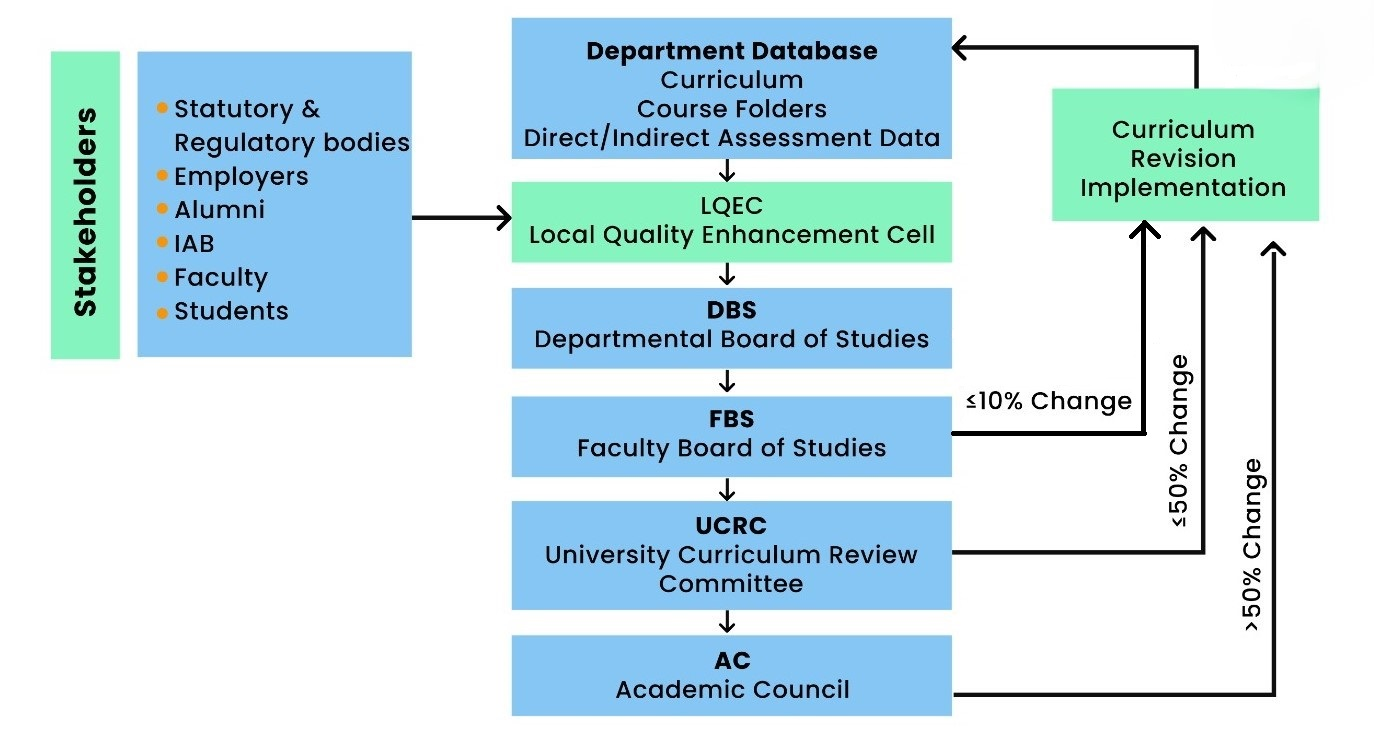
\includegraphics[width=0.92\textwidth]{images/criterion_8/media/Curr_review.jpeg} \caption{Processes for Curriculum Review} \label{figure:pfcr} \end{figure} 

The curriculum is composed of a balanced combination of engineering and non-engineering domains coupled with appropriate assessment and evaluation methods. The program curriculum involves both theory and laboratory work through all three learning domains of Bloom's Taxonomy. The cognitive, psychomotor, and affective domains cover 74\%, 15\% and 11\% of the curriculum, respectively, as shown in Figure~\ref{figure:percentage_bloom_taxonomy}.
\begin{figure}[!h]
    \centering
    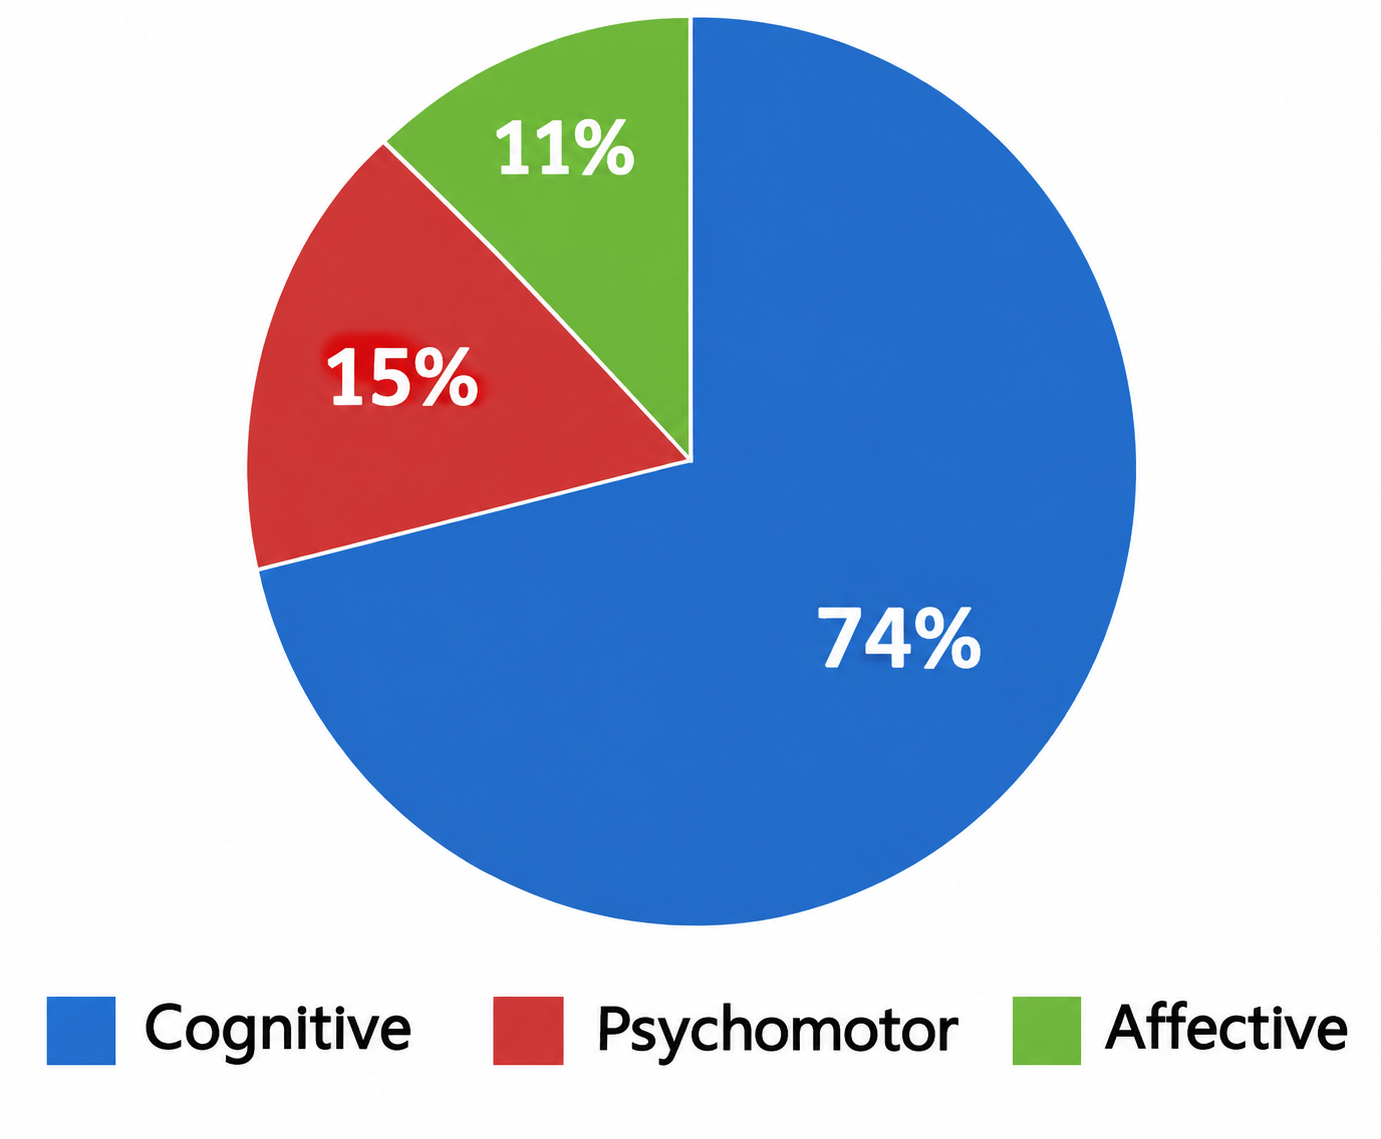
\includegraphics[width=0.50\textwidth]{images/criterion_3/media/BT-Domains.png}
    \caption{Percentage of Learning Domains of Bloom's Taxonomy}
    \label{figure:percentage_bloom_taxonomy}
\end{figure}
%\begin{comment}
%\begin{figure}[H]
%\centering
%\includegraphics[width=0.92\textwidth]{images/criterion_3/media/image10.png}
%\caption{Figure 4.2: Program Structure Outline}
%\end{figure}
%\end{comment}
The curriculum developed for BESE Program at NUST-SEECS also encompasses the national requirements based on engineering and non-engineering areas. The distribution of courses for BESE program at SEECS is shown in Annexure~\ref{app:criteria3-intake-2k25-wp30} (WP No.30-72nd  ACM-04 Sep 2025). It also presents the distribution of courses as per knowledge area in Software Engineering program at SEECS.

\begin{comment}
The SEECS program is benchmarked against international software engineering programs by comparing credit hours across engineering and non-engineering knowledge area domains. Table~\ref{tab:Comparison_of_Credits_of_SEECS_Program_with_International_Programs_in_Software_Engineering} shows the number of credits in each domain subdivided into subject areas, giving a comprehensive comparison with universities running a semester system.
The SEECS BESE program is benchmarked against international software engineering programs by comparing engineering and non-engineering credit hours across subject areas (Table~\ref{tab:Comparison_of_Credits_of_SEECS_Program_with_International_Programs_in_Software_Engineering}), showing strong alignment with universities using the semester system. This alignment is further illustrated in Figure~\ref{figure:Comparison_of_credits_of_SEECS_BESE_program_and_international_programs} through a histogram comparison of engineering and non-engineering credits.

\begin{figure}[H]
\centering
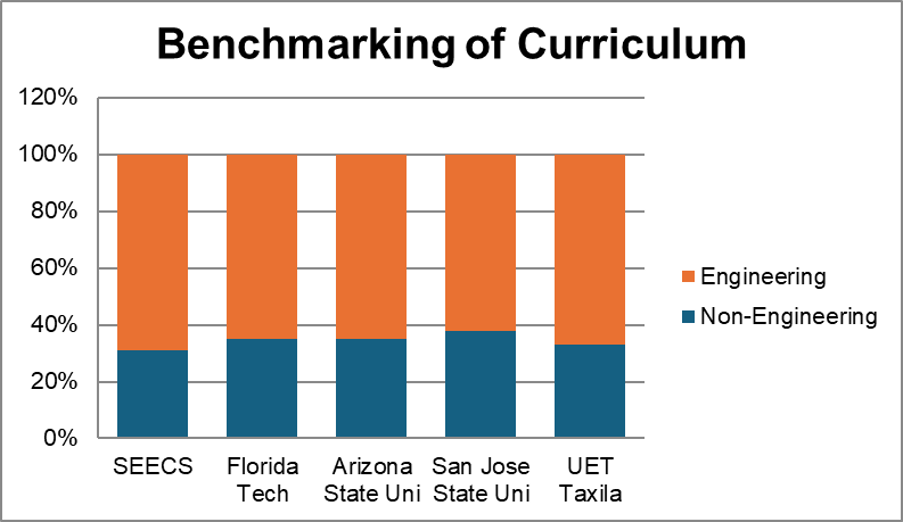
\includegraphics[width=\textwidth]{images/criterion_3/media/img_benchmarking_curriculum.png}
\caption{Comparison of credits of SEECS BESE program and international programs}
\label{figure:Comparison_of_credits_of_SEECS_BESE_program_and_international_programs}
\end{figure}

\clearpage
\begin{landscape}
\begingroup\scriptsize\setlength{\tabcolsep}{3pt}
\begin{longtable}{>{\raggedright\arraybackslash}p{0.12\linewidth}
                  >{\raggedright\arraybackslash}p{0.22\linewidth}
                  >{\centering\arraybackslash}p{0.08\linewidth}
                  >{\centering\arraybackslash}p{0.09\linewidth}
                  >{\centering\arraybackslash}p{0.10\linewidth}
                  >{\centering\arraybackslash}p{0.10\linewidth}
                  >{\centering\arraybackslash}p{0.09\linewidth}}
\caption{Comparison of Credits of SEECS Program with International Programs in Software Engineering} \\ 
\label{tab:Comparison_of_Credits_of_SEECS_Program_with_International_Programs_in_Software_Engineering}
\toprule
\textbf{Domain} & \textbf{Knowledge Area} & \textbf{SEECS} & \textbf{Florida Tech} & \textbf{Arizona State Uni} & \textbf{San Jose State Uni} & \textbf{UET Taxila} \\
\midrule
\endfirsthead
\multicolumn{7}{l}{\footnotesize\textit{Continued from previous page}} \\
\toprule
\textbf{Domain} & \textbf{Knowledge Area} & \textbf{SEECS} & \textbf{Florida Tech} & \textbf{Arizona State Uni} & \textbf{San Jose State Uni} & \textbf{UET Taxila} \\
\midrule
\endhead
\bottomrule
\endlastfoot
\textbf{Non-Engineering} & Humanities & 18 & 18 & 18 & 24 & 16 \\
 & Management Sciences & 5 & 0 & 0 & 0 & 12 \\
 & Natural Sciences & 18 & 25 & 23 & 21 & 14 \\
 & Community Service Learning & 2 & 1 & 1 & 0 & 2 \\
 & \textbf{Sub Total} & \textbf{43 (31\%)} & \textbf{44 (35\%)} & \textbf{42 (35\%)} & \textbf{45 (38\%)} & \textbf{44 (33\%)} \\
\addlinespace
\textbf{Engineering} & Computing & 7 & 10 & 15 & 13 & 25 \\
 & Engineering Foundation & 27 & 21 & 18 & 15 & 18 \\
 & Major Based Core (Breadth) & 30 & 18 & 21 & 23 & 20 \\
 & Major Based Core (Depth) & 18 & 12 & 15 & 15 & 17 \\
 & Inter-Disciplinary Eng. Breadth (Electives) & 7 & 15 & 3 & 3 & 3 \\
 & Senior Design Project & 6 & 6 & 6 & 5 & 6 \\
 & \textbf{Sub Total} & \textbf{95 (69\%)} & \textbf{82 (65\%)} & \textbf{78 (65\%)} & \textbf{75 (62\%)} & \textbf{89 (67\%)} \\
\addlinespace
\textbf{Total} & & \textbf{138} & 126 & 120 & 120 & 133 \\
\end{longtable}
\endgroup
\end{landscape}
\end{comment}

%\begin{figure}[H]
%\centering
%\includegraphics[width=0.81\textwidth]{images/criterion_3/media/image8.png}
%\caption{Figure 4.4b: Comparison of Credits (Note: Internship in summer for qualifying)}
%\end{figure}

Curriculum revision is a continuous process, and the Table~\ref{tab:Revision_of_BESE_Curriculum} shows the curriculum revision timeline since 2023.
\begin{table}[htbp]
\centering
\footnotesize % <-- Reduces font size
\renewcommand{\arraystretch}{0.85} % <-- Tightens vertical row spacing
\caption{Curriculum Revision Timeline}
\label{tab:Revision_of_BESE_Curriculum}
\begin{tabular}{c >{\raggedright\arraybackslash}p{0.36\textwidth} >{\raggedright\arraybackslash}p{0.46\textwidth}}
\toprule
\textbf{Ser\#} & \textbf{Working Paper (WP)} & \textbf{Description} \\
\midrule

1 & Curriculum (WP No.30--72\textsuperscript{nd} ACM-04 Sep 2025) 
  & Latest revision of BE Software Engg \newline 
    Applicable from BESE 2025 (intake Fall 2025) \newline 
    Annexure~\ref{app:criteria3-intake-2k25-wp30} \\ \addlinespace

2 & Curriculum (WP No.20--69\textsuperscript{th} ACM-06 Aug 2024) 
  & Revision of BE Software Engg \newline 
    Applicable from BESE 2024 (intake Fall 2024) \newline 
    Annexure~\ref{app:criteria-3_intake-2k24-wp20} \\ \addlinespace

3 & Curriculum (WP No.30--64\textsuperscript{th} ACM-23 Jan 2023) 
  & Revision of BE Software Engg \newline 
    Applicable from BESE 2019 (intake Fall 2019) \newline 
    Annexure~\ref{app:criteria-3_intake-2K19-wp30} \\

\bottomrule
\end{tabular}
\end{table}
The BESE program spans four years and is currently based primarily on the curriculum approved by PEC in 2020. WP No.30--64th ACM-23 Jan 2023 (Annexure~\ref{app:criteria-3_intake-2K19-wp30}) revised the FYDP credit distribution in the 7th and 8th semesters from 3 CHs each to 2 CHs and 4 CHs, respectively, to meet the minimum regular semester load. WP No.20--69th ACM-06 Aug 2024 (Annexure~\ref{app:criteria-3_intake-2k24-wp20}) aligned the BESE curriculum with PEC Engineering Education Guidelines for adopting HEC UEP-2023 (EC letter no. 15-54/Coord/2019/HEC/(CURR/UEP)/578, July 13, 2023), incorporating prescribed English courses, replacing Pakistan Studies with Ideology and Constitution of Pakistan, introducing Ethics for non-Muslim students, and adjusting semester-wise credit hour distribution within approved limits.

Subsequently, PEC issued latest guidelines (letter no. PEC/AD/CD/2025/03, April 10, 2025) for incorporating HEC UEP-2024, mandating compulsory courses such as Pakistan Studies, Fehm-e-Quran-I, and Fehm-e-Quran-II within the General Education/Non-Engineering domain effective Fall 2025. Accordingly, a revised BESE curriculum was proposed and approved in the 72nd ACM-04 Sep 2025 (Annexure~\ref{app:criteria3-intake-2k25-wp30}) to align with the updated PEC framework.

The department regularly obtains feedback from industry stakeholders through the Industrial Advisory Board (IAB). The feedback is reviewed by the department and considered as an important input for the continuous improvement and revision of the curriculum. Based on identified needs and emerging trends in the software engineering profession, appropriate changes are incorporated to enhance curriculum relevance, strengthen technical competencies, and address the evolving requirements of industry. The recommendations and their implementation are documented and monitored through the established academic review and approval mechanisms.

\begin{comment}
\begin{table}[htbp]
\centering
\caption{Revision of BESE Curriculum} % <--- Caption added here
\label{tab:Revision_of_BESE_Curriculum}                       % <--- Added label for referencing
\vspace{0.2cm}                                   % Adds spacing between caption and table
\begin{tabular}{|c|p{5cm}|p{7.5cm}|}
\hline
\rowcolor[gray]{0.7} 
\textbf{Ser\#} & \textbf{Working Paper (WP)} & \textbf{Description} \\ \hline

1 & Curriculum (WP No.30--72\textsuperscript{nd} ACM-04 Sep 2025) 
  & Revision of BE Software Engg \newline 
    Applicable from BESE 2025 (intake Fall 2025) \newline 
    Annex 3.1 \\ \hline

2 & Curriculum (WP No.20--69\textsuperscript{th} ACM-06 Aug 2024 ) 
  & Revision of BE Software Engg \newline 
    Applicable from BESE 2024 (intake Fall 2024) \newline 
    Annex 3.2 \\ \hline

2 & Curriculum (WP No.30--64\textsuperscript{th} ACM- 23 Jan 2023) 
  & Revision of BE Software Engg \newline 
    Applicable from BESE 2019 onward (intake Fall 2019) Annex 3.3 \\ \hline
\end{tabular}
\end{table}
\end{comment}

The revised distribution as per WP No.30-64\textsuperscript{th}th ACM-23 Jan 2023 (Annexure~\ref{app:criteria-3_intake-2K19-wp30})(BESE 2K19-2K23), and WP No. 20 -69th ACM-06 Aug 2024 (BESE-2K24) (Annexure~\ref{app:criteria-3_intake-2k24-wp20}) in accordance with PEC revised curriculum is presented in the Table~\ref{tab:BESE_Curriculum_(Applicable_on_2021–2024_Intakes)_vs._PEC_Curriculum_2020}. The proposed revisions as per WP~\#30, 72\textsuperscript{nd} ACM in accordance with UGEP and HEC guidelines are presented in Table~\ref{tab:BESE_Curriculum_Intake_2025} and Table~\ref{tab:BESE_Curriculum_Intake_2025_onward}.

\begin{landscape}
\begingroup\scriptsize\setlength{\tabcolsep}{3pt}
\begin{longtable}{>{\raggedright\arraybackslash}p{0.12\linewidth}
                  >{\raggedright\arraybackslash}p{0.11\linewidth}
                  >{\raggedright\arraybackslash}p{0.16\linewidth}
                  >{\centering\arraybackslash}p{0.07\linewidth}
                  >{\centering\arraybackslash}p{0.09\linewidth}
                  >{\centering\arraybackslash}p{0.07\linewidth}
                  >{\centering\arraybackslash}p{0.09\linewidth}
                  >{\centering\arraybackslash}p{0.07\linewidth}
                  >{\centering\arraybackslash}p{0.09\linewidth}}
\caption{BESE Curriculum (Applicable on 2019--2024 Intakes) vs.\ PEC Curriculum 2020} \\
\label{tab:BESE_Curriculum_(Applicable_on_2021–2024_Intakes)_vs._PEC_Curriculum_2020} \\
\toprule
\textbf{Domain} & \textbf{WK Category} & \textbf{Knowledge Area} & \multicolumn{2}{c}{\textbf{Core}} & \multicolumn{2}{c}{\textbf{Elective}} & \multicolumn{2}{c}{\textbf{Total}} \\
& & & \textbf{PEC} & \textbf{NUST SEECS} & \textbf{PEC} & \textbf{NUST SEECS} & \textbf{PEC} & \textbf{NUST SEECS} \\
\midrule
\endfirsthead
\multicolumn{9}{l}{\footnotesize\textit{Continued from previous page}} \\
\toprule
\textbf{Domain} & \textbf{WK Category} & \textbf{Knowledge Area} & \textbf{PEC Core} & \textbf{SEECS Core} & \textbf{PEC Elec.} & \textbf{SEECS Elec.} & \textbf{PEC Total} & \textbf{SEECS Total} \\
\midrule
\endhead
\bottomrule
\endlastfoot
\textbf{Engineering Domain} & WK-2/4/5/6 & Computing and Information Science & 6 & 7 & --- & --- & \textbf{6} & \textbf{7} \\
 & WK-3/2 & Engineering Foundation & 30 & 30 & - & --- & \textbf{30} & \textbf{30} \\
 & WK-4/2/1 & Software Engg.\ Core Breadth & 27 & 27 & - & --- & \textbf{27} & \textbf{27} \\
 & WK-5/6 & Software Engg.\ Core Depth & --- & --- & 18 & 18+X & \textbf{18} & \textbf{18+X} \\
 & WK-6/7/8 & Final Year Design Project & 6 & 6 & --- & --- & \textbf{6} & \textbf{6} \\
 & WK-3/4/2/1 & Multi-Disciplinary Engineering Electives & 1 & 1 & 6 & 6 & \textbf{7} & \textbf{7} \\
\addlinespace
\textbf{Non-Engineering Domain} & WK-7 & Humanities & 11 & 10 & --- & --- & \textbf{11} & \textbf{10} \\
 & --- & Social Sciences & --- & --- & 4 & 4 & \textbf{4} & \textbf{4} \\
 & --- & Management Sciences & --- & --- & 5 & 5 & \textbf{5} & \textbf{5} \\
 & WK-1 & Natural Sciences & 4 & 3 & - & - & \textbf{4} & \textbf{3} \\
 & WK-2 & Mathematics & 15 & 15 & - & - & \textbf{15} & \textbf{15} \\
 & WK-7 & Civic \& Community Engagement & 0 & 2 & --- & --- & \textbf{0} & \textbf{2} \\
\addlinespace
\textbf{Total} & & & & & & & \textbf{133} & \textbf{134+X} \\
\end{longtable}
\endgroup
\end{landscape}


\begin{landscape}
\begingroup\scriptsize\setlength{\tabcolsep}{3pt}
\begin{longtable}{>{\raggedright\arraybackslash}p{0.12\linewidth}
                  >{\raggedright\arraybackslash}p{0.11\linewidth}
                  >{\raggedright\arraybackslash}p{0.16\linewidth}
                  >{\centering\arraybackslash}p{0.07\linewidth}
                  >{\centering\arraybackslash}p{0.09\linewidth}
                  >{\centering\arraybackslash}p{0.07\linewidth}
                  >{\centering\arraybackslash}p{0.09\linewidth}
                  >{\centering\arraybackslash}p{0.07\linewidth}
                  >{\centering\arraybackslash}p{0.09\linewidth}}
\caption{BESE Curriculum (Intake 2025 \& Onwards) vs.\ PEC Curriculum 2020 -- Core and Elective Focused} \\
\label{tab:BESE_Curriculum_Intake_2025} \\
\toprule
\textbf{Domain} & \textbf{WK Category} & \textbf{Knowledge Area} & \multicolumn{2}{c}{\textbf{Core}} & \multicolumn{2}{c}{\textbf{Elective}} & \multicolumn{2}{c}{\textbf{Total}} \\
& & & \textbf{PEC} & \textbf{NUST SEECS} & \textbf{PEC} & \textbf{NUST SEECS} & \textbf{PEC} & \textbf{NUST SEECS} \\
\midrule
\endfirsthead
\multicolumn{9}{l}{\footnotesize\textit{Continued from previous page}} \\
\toprule
\textbf{Domain} & \textbf{WK Cat.} & \textbf{Knowledge Area} & \textbf{PEC Core} & \textbf{SEECS Core} & \textbf{PEC Elec.} & \textbf{SEECS Elec.} & \textbf{PEC Total} & \textbf{SEECS Total} \\
\midrule
\endhead
\bottomrule
\endlastfoot
\textbf{Engineering Domain} & WK-2/4/5/6 & Computing and Information Science & 6 & 7 & --- & --- & \textbf{6} & \textbf{7} \\
 & WK-3/2 & Engineering Foundation & 30 & 30 & - & --- & \textbf{30} & \textbf{30} \\
 & WK-4/2/1 & Software Engg.\ Core Breadth & 27 & 27 & - & --- & \textbf{27} & \textbf{27} \\
 & WK-5/6 & Software Engg.\ Core Depth & --- & --- & 18 & 18+X & \textbf{18} & \textbf{18+X} \\
 & WK-6/7/8 & Final Year Design Project & 6 & 6 & --- & --- & \textbf{6} & \textbf{6} \\
 & WK-3/4/2/1 & Multi-Disciplinary Engineering Electives & 1 & 1 & 6 & 6 & \textbf{7} & \textbf{7} \\
\addlinespace
\textbf{Non-Engineering Domain} & WK-7 & Humanities & 11 & 14 & --- & --- & \textbf{11} & \textbf{14} \\
 & --- & Social Sciences & --- & --- & 4 & 4 & \textbf{4} & \textbf{4} \\
 & --- & Management Sciences & --- & --- & 5 & 5 & \textbf{5} & \textbf{5} \\
 & WK-1 & Natural Sciences & 4 & 3 & - & - & \textbf{4} & \textbf{3} \\
 & WK-2 & Mathematics & 15 & 15 & - & - & \textbf{15} & \textbf{15} \\
 & WK-7 & Civic \& Community Engagement & 0 & 2 & --- & --- & \textbf{0} & \textbf{2} \\
\addlinespace
\textbf{Total} & & & & & & & \textbf{133} & \textbf{138+X} \\
\end{longtable}
\endgroup
\end{landscape}

\begin{comment}
%\end{gather}
\begin{table}[H]
\centering
\caption{BESE Curriculum (BESE 2025 \& Onwards) vs.\ PEC Curriculum}
\label{tab:BESE_Curriculum_Intake_2025_onward}
\begin{tabular}{>{\raggedright\arraybackslash}p{0.15\textwidth}
                >{\raggedright\arraybackslash}p{0.30\textwidth}
                >{\centering\arraybackslash}p{0.10\textwidth}
                >{\centering\arraybackslash}p{0.07\textwidth}
                >{\centering\arraybackslash}p{0.10\textwidth}
                >{\centering\arraybackslash}p{0.07\textwidth}}
\toprule
\multicolumn{6}{l}{\textbf{Curriculum Design (Fall 2025 and Onwards Batches)}} \\
\midrule
\textbf{Domain} & \textbf{Knowledge Area} & \multicolumn{2}{c}{\textbf{PEC Recommended}} & \multicolumn{2}{c}{\textbf{Institute's Program}} \\
& & \textbf{Total Credits} & \textbf{Overall \%} & \textbf{Total Credits} & \textbf{Overall \%} \\
\midrule
\textbf{Non-Engineering} & Humanities & 11 & \textbf{29.3\%} & 14 & \textbf{31.1\%} \\
 & Social Sciences & 4 & & 4 & \\
 & Management Sciences & 5 & & 5 & \\
 & Natural Sciences & 19 & & 18 & \\
 & Civic \& Community Engagement & --- & & 2 & \\
 & \textbf{Sub Total} & \textbf{39} & & \textbf{43} & \\
\addlinespace
\textbf{Engineering} & Computing & 6 & \textbf{70.7\%} & 7 & \textbf{68.9\%} \\
 & Engineering Foundation & 30 & & 30 & \\
 & Major Based Core (Breadth) & 27 & & 27 & \\
 & Major Based Core (Depth) & 18 & & 18+X & \\
 & Inter-Disciplinary Eng.\ Breadth (Electives) & 7 & & 7 & \\
 & Senior Design Project & 6 & & 6 & \\
 & Industrial Training (Summer) & 0 & & 0 & \\
 & \textbf{Sub Total} & \textbf{94} & & \textbf{95+X} & \\
\addlinespace
\textbf{Total} & & \textbf{133} & \textbf{100\%} & \textbf{138+X} & \textbf{100\%} \\
\bottomrule
\end{tabular}
\end{table}
\end{comment}

\begin{table}[H]
\centering
\footnotesize % <-- Reduces font size further
\renewcommand{\arraystretch}{0.85} % <-- Reduces row height/vertical padding
\caption{BESE Curriculum (BESE 2025 \& Onwards) vs.\ PEC Curriculum 2020}
\label{tab:BESE_Curriculum_Intake_2025_onward}
\begin{tabular}{>{\raggedright\arraybackslash}p{0.15\textwidth}
                >{\raggedright\arraybackslash}p{0.28\textwidth}
                >{\centering\arraybackslash}p{0.10\textwidth}
                >{\centering\arraybackslash}p{0.07\textwidth}
                >{\centering\arraybackslash}p{0.10\textwidth}
                >{\centering\arraybackslash}p{0.07\textwidth}}
\toprule
\multicolumn{6}{l}{\textbf{Curriculum Design (Fall 2025 and Onwards Batches)}} \\
\midrule
\textbf{Domain} & \textbf{Knowledge Area} & \multicolumn{2}{c}{\textbf{PEC Recommended}} & \multicolumn{2}{c}{\textbf{Institute's Program}} \\
& & \textbf{Total Credits} & \textbf{Overall \%} & \textbf{Total Credits} & \textbf{Overall \%} \\
\midrule
\textbf{Non-Engineering} & Humanities & 11 &  & 14 &  \\
 & Social Sciences & 4 & & 4 & \\
 & Management Sciences & 5 & & 5 & \\
 & Natural Sciences (including Maths) & 19 & & 18 & \\
 & Civic \& Community Engagement & --- & & 2 & \\
 & \textbf{Sub Total} & \textbf{39} & \textbf{29.3\%} & \textbf{43} & \textbf{31.1\%}\\
\addlinespace
\textbf{Engineering} & Computing & 6 &  & 7 &\\
 & Engineering Foundation & 30 & & 30 & \\
 & Major Based Core (Breadth) & 27 & & 27 & \\
 & Major Based Core (Depth) & 18 & & 18+X & \\
 & Inter-Disciplinary Eng.\ Breadth (Electives) & 7 & & 7 & \\
 & Senior Design Project & 6 & & 6 & \\
 & Industrial Training (Summer) & 0 & & 0 & \\
 & \textbf{Sub Total} & \textbf{94} & \textbf{70.7\%}& \textbf{95+X} &  \textbf{68.9\%} \\
\addlinespace
\textbf{Total} & & \textbf{133} & \textbf{100\%} & \textbf{138+X} & \textbf{100\%} \\
\bottomrule
\end{tabular}
\end{table}

For comprehensive achievement of BESE curriculum and all its related activities, well-defined time intervals are allocated, referred as “Credit-Hour.” One credit hour represents one contact hour a week in class or three contact hours a week of laboratory work per semester. 

\hypertarget{sec:4.7delivery}{%
\section{Delivery and Assessment Methods}\label{sec:4.7delivery}}

A broad range of teaching and assessment methods are incorporated into course outlines, designed to enable students to meet outcomes outlined in the CLOs. Students develop and practice skills through presentations and group-based cooperative learning. Program delivery covers the three learning domains of Bloom's Taxonomy (Figure~\ref{figure:percentage_bloom_taxonomy}) through theoretical coursework, laboratory work and FYDP addressing complex engineering problems.

\hypertarget{sec:4.2.1coursework}{%
\subsection{Course Work}\label{sec:4.2.1coursework}}

The BESE program at SEECS has a comprehensive system for planning and monitoring curriculum delivery. At the start of each semester, the program coordinator allocates courses and develops a delivery schedule (Timetable). Faculty prepares a detailed course outlines and submits to the Knowledge Group Head (KGH) for quality review and approval (vetted sample in Annexure~\ref{app:criteria-3_Course Outline with Knowledge Group Head's Signature}). CLOs remain constant unless revised through prescribed CQI process. Each CLO is mapped on a respective PLO to attribute the PLO attainment at the program level. Course outlines, CLOs, and assessment/action plans (Figure~\ref{figure:course_assessment_criteria}) are shared with students by the first week of the semester via Qalam and LMS. Both are regularly updated with relevant course content and marks obtained in assessments as the semester progresses. 

\begin{figure}[H]
\centering
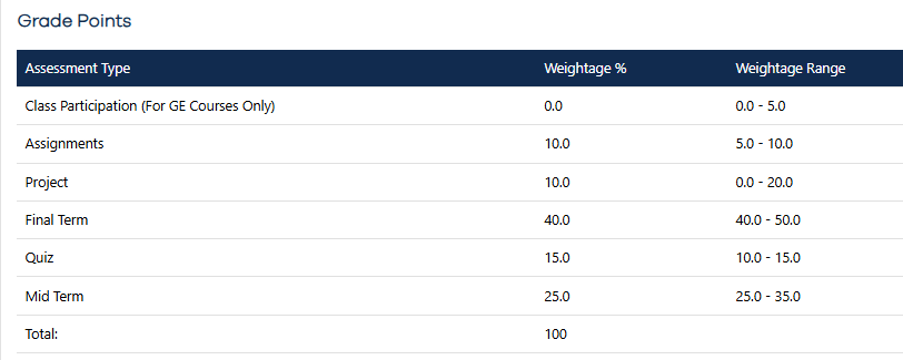
\includegraphics[width=0.97\textwidth]{images/criterion_3/media/img_course_assessment_criteria.png}
\caption{Course Assessment Criteria}
\label{figure:course_assessment_criteria}
\end{figure}

Each semester is planned to facilitate 16 weeks of teaching and 2 weeks of examination (MSE and ESE). A sample semester planner is shown in Figure~\ref{fig:planner}. Detailed data on the system of instructions and examination is given in Annexure~\ref{app:criteria-3_System of instruction and examination}. Assessment activities are distributed across the semester and their frequency is determined by the course credit hours. Generally for a course with 3 credit hours 5-6 quizzes are taken, while for a 2 credit hours course 3-4 quizzes are conducted. Similarly, 1 assignment per credit hour is taken throughout the semester. There is only one Mid Semester and one End Semester Exam per course. A semester project is usually assigned to the students in each course especially the engineering ones. For General Education courses, class participation has a mandatory weightage upto 5\%. 

All classes and labs are conducted via on-campus face-to-face mode. However, under unavoidable circumstances (i.e. lockdown etc.) the institute has online readiness capabilities via MS-Teams.

\begin{figure}[H]
\centering
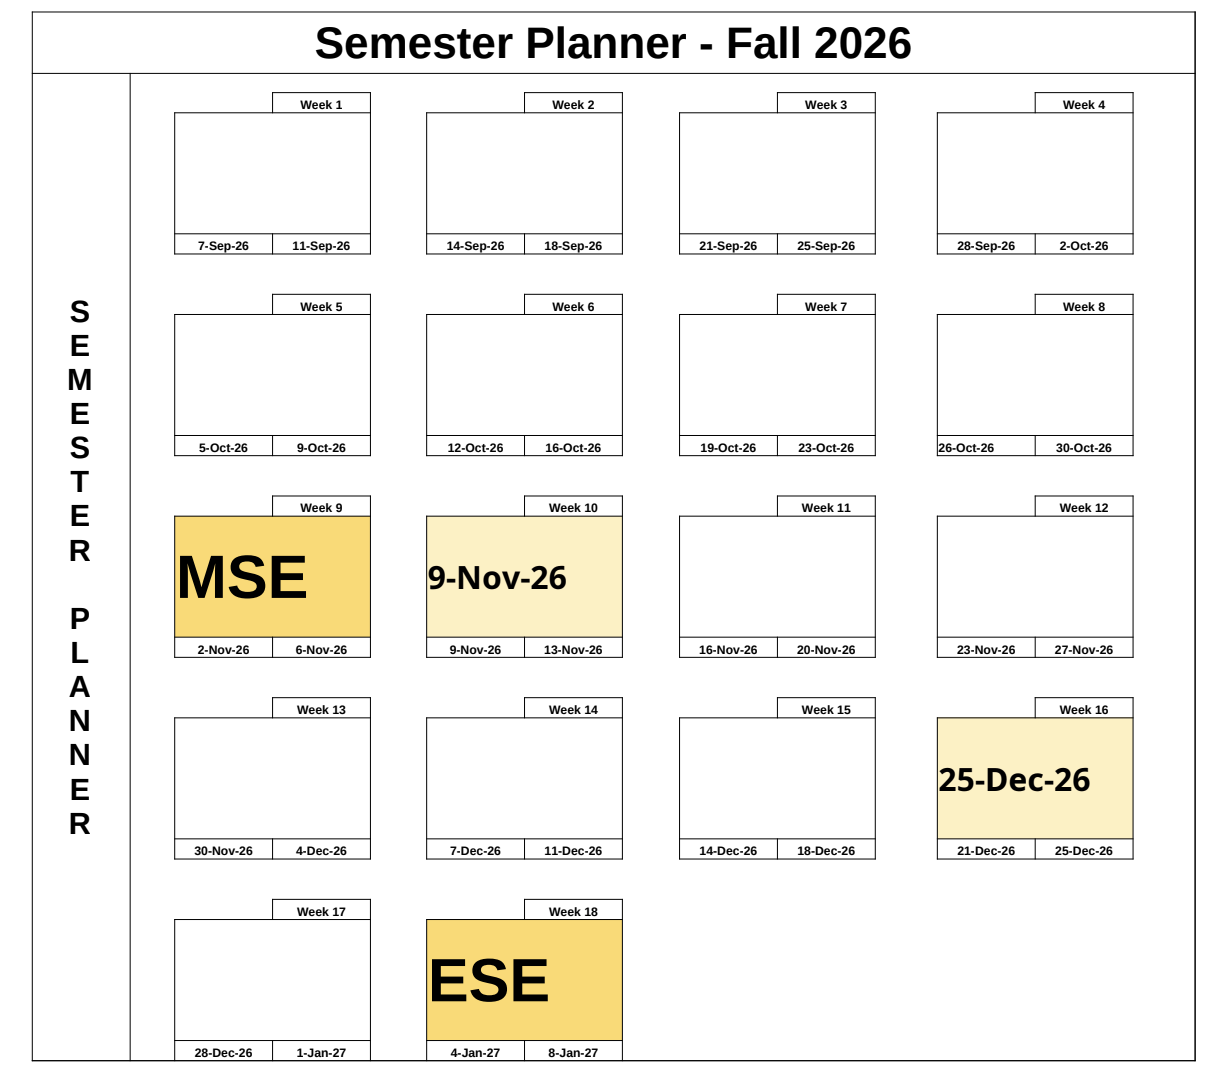
\includegraphics[width=0.97\textwidth]{images/criterion_3/media/planner.png}
\caption{Sample Semester Planner}
\label{fig:planner}
\end{figure}

%\hypertarget{sec:4.2.2coursework}{%
%\subsection{Assessment of CLOs and PLOs}\label{sec:4.2.2coursework}}

\hypertarget{sec:4.4labwork}{%
\subsection{Laboratory Work}\label{sec:4.4labwork}}

NUST-SEECS has state-of-the-art laboratories to support the Software Engineering curriculum requirements.  These laboratories are equipped with modern computing facilities and reliable networking infrastructure to support a wide range of academic and practical activities. 

\hypertarget{sec:labassessment}{%
\subsubsection{Lab Assessment}\label{sec:labassessment}}

There are at least 2 or more lab courses offered in each semester. The content of each lab from a specific course is carefully designed to meet the needs of the course and to achieve the CLOs defined for the course. The list of lab experiments for CS-368 Reinforcement Learning course is given in Table~\ref{tab:List_of_Lab_Experiments_for_CS_368_Reinforcement_Learning} as an example.

\begin{table}[H]
\centering
\small % <-- Reduces font and table size
\caption{List of Lab Experiments for CS-368 Reinforcement Learning}
\label{tab:List_of_Lab_Experiments_for_CS_368_Reinforcement_Learning}
\begin{tabular}{>{\centering\arraybackslash}p{0.12\textwidth}
                >{\raggedright\arraybackslash}p{0.62\textwidth}
                >{\centering\arraybackslash}p{0.20\textwidth}}
\toprule
\textbf{Lab No.} & \textbf{Lab Experiment} & \textbf{CLO} \\
\midrule
Lab 1  & Introduction to NumPy Library & CLO-1 / CLO-4 \\
Lab 2  & Data Visualization in Python & CLO-1 / CLO-4 \\
Lab 3  & Markov Decision Processes -- Iterative Policy Evaluation, Policy Iteration, Value Iteration & CLO-1 / CLO-4 \\
Lab 4  & Monte Carlo \& TD Learning -- Prediction [Cliff Walking \& Frozen Lake Env.] & CLO-1 / CLO-4 \\
Lab 5  & n-Step TD and TD($\lambda$) -- Prediction [Frozen Lake \& Taxi Environments] & CLO-1 / CLO-4 \\
Lab 6  & SARSA -- Control [Cart Pole \& Acrobat Environments] & CLO-1 / CLO-4 \\
Lab 7  & n-Step SARSA \& SARSA($\lambda$) -- Control [Cart Pole \& Pendulum Environments] & CLO-1 / CLO-4 \\
Lab 8  & Q-Learning \& Double Q-Learning -- Control [Mountain Car \& Lunar Lander Environments] & CLO-1 / CLO-4 \\
Lab 9  & Deep Q Networks -- I [Acrobat Environment] & CLO-1 / CLO-4 \\
Lab 10 & Deep Q Networks -- II (Stable Baselines3) [Lunar Lander \& Blackjack Environments] & CLO-1 / CLO-4 \\
Lab 11 & Advantage Actor Critic (A3C) [Bipedal Walker \& Car Racing Environments] & CLO-1 / CLO-4 \\
Lab 12 & Proximal Policy Optimization (PPO) [Pendulum \& Taxi Environments] & CLO-1 / CLO-4 \\
Lab 13 & Soft Actor Critic (SAC) [Blackjack Environment] & CLO-1 / CLO-4 \\
Lab 14 & Open Ended Lab [MuJoCo Environment] & CLO-1 / CLO-4 \\
Lab 15 & Project [Atari Environments] & CLO-2 / CLO-3 / CLO-4 \\
Lab 16 & Project [Atari Environments] & CLO-2 / CLO-3 / CLO-4 \\
\bottomrule
\end{tabular}
\end{table}

The Lab work is evaluated according to the criteria shown in Figure~\ref{figure:lab_assessment_criteria}.

\begin{figure}[H]
\centering
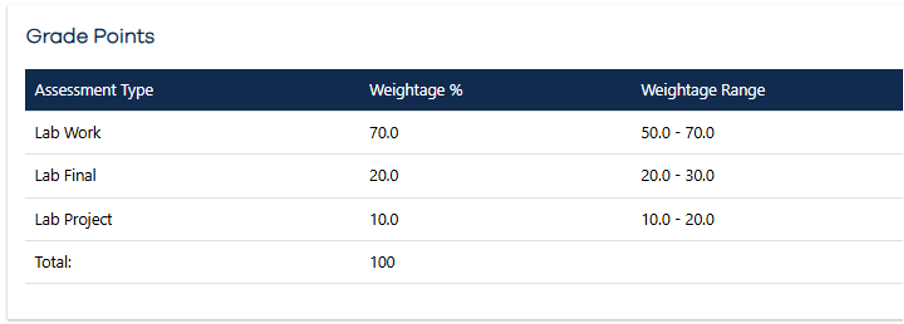
\includegraphics[width=0.97\textwidth]{images/criterion_3/media/img_lab_assessment_criteria.png}
\caption{Lab Assessment Criteria}
\label{figure:lab_assessment_criteria}
\end{figure}

Students are required to work individually or in teams of 2--3 members to accomplish practical tasks ranging from guided responses to open-ended problems. The lab folder is maintained on the LMS of NUST-SEECS. It is a comprehensive soft-copy record of all labs offered and managed by the faculty teaching the course. A sample lab manual of CS-415 Mobile Application Development (Lab~6) is given in Annexure~\ref{app:criteria-3_Sample Lab Manual}.  The lab folder in conjunction with the course folder assists academic staff in proper documentation.

\begin{comment}
\begin{table}[H]
\centering
\caption{List of Lab Experiments for CS-368 Reinforcement Learning}
\label{tab:List_of_Lab_Experiments_for_CS_368_Reinforcement_Learning}
\begin{tabular}{>{\centering\arraybackslash}p{0.10\textwidth}
                >{\raggedright\arraybackslash}p{0.74\textwidth}
                >{\centering\arraybackslash}p{0.11\textwidth}}
\toprule
\textbf{Lab No.} & \textbf{Lab Experiment} & \textbf{CLO} \\
\midrule
Lab 1  & Introduction to NumPy Library & CLO-1 / CLO-4 \\
Lab 2  & Data Visualization in Python & CLO-1 / CLO-4 \\
Lab 3  & Markov Decision Processes -- Iterative Policy Evaluation, Policy Iteration, Value Iteration & CLO-1 / CLO-4 \\
Lab 4  & Monte Carlo \& TD Learning -- Prediction [Cliff Walking \& Frozen Lake Env.] & CLO-1 / CLO-4 \\
Lab 5  & n-Step TD and TD($\lambda$) -- Prediction [Frozen Lake \& Taxi Environments] & CLO-1 / CLO-4 \\
Lab 6  & SARSA -- Control [Cart Pole \& Acrobat Environments] & CLO-1 / CLO-4 \\
Lab 7  & n-Step SARSA \& SARSA($\lambda$) -- Control [Cart Pole \& Pendulum Environments] & CLO-1 / CLO-4 \\
Lab 8  & Q-Learning \& Double Q-Learning -- Control [Mountain Car \& Lunar Lander Environments] & CLO-1 / CLO-4 \\
Lab 9  & Deep Q Networks -- I [Acrobat Environment] & CLO-1 / CLO-4 \\
Lab 10 & Deep Q Networks -- II (Stable Baselines3) [Lunar Lander \& Blackjack Environments] & CLO-1 / CLO-4 \\
Lab 11 & Advantage Actor Critic (A3C) [Bipedal Walker \& Car Racing Environments] & CLO-1 / CLO-4 \\
Lab 12 & Proximal Policy Optimization (PPO) [Pendulum \& Taxi Environments] & CLO-1 / CLO-4 \\
Lab 13 & Soft Actor Critic (SAC) [Blackjack Environment] & CLO-1 / CLO-4 \\
Lab 14 & Open Ended Lab [MuJoCo Environment] & CLO-1 / CLO-4 \\
Lab 15 & Project [Atari Environments] & CLO-2 / CLO-3 / CLO-4 \\
Lab 16 & Project [Atari Environments] & CLO-2 / CLO-3 / CLO-4 \\
\bottomrule
\end{tabular}
\end{table}
\end{comment}



\hypertarget{sec:labrubrics}{%
\subsubsection{Lab Rubrics}\label{sec:labrubrics}}

\begin{comment}
During the CQI process, the process for creating lab rubrics has been revised to address inconsistencies in rubric application across lab assessments in core depth and breadth courses. The essential requirements for the lab rubrics process are:

\begin{enumerate}[label=\alph*.]
\item Each lab for a given course must have a rubric on which the student's work can be evaluated.
\item The rubric may have one or more evaluation criteria (rubric items) to assess different outcomes associated with the lab.
\item Each rubric item must have at least three levels defined to categorize a student's work based on quality.
\item Each rubric item must have a one-to-one mapping to a CLO for the given course. Any rubric item without a corresponding CLO should be removed.
\item Each rubric item should assess the learning outcomes associated with the corresponding CLO and consequently the PLO.
\item For rubric items that use the psychomotor or affective domain, appropriate descriptors should be used and observation evidence must be maintained.
\item Once the rubric is finalized, approval is required from the faculty member and the Knowledge Group Head (KGH) to track the CQI process.
\end{enumerate}
\end{comment}

Lab works are evaluated using structured rubrics to ensure consistent  and objective assessment of students' practical performance. The attainment of CLOs and PLOs for lab/practical work is also done through these rubrics. An example of a lab rubric is given in Annexure~\ref{app:criteria-3_Lab Rubric Based Evaluation}. The lab rubrics are designed in accordance with the relevant levels of Bloom's Taxonomy, assessing students' understanding, analysis, and problem-solving skills through practical tasks. 

\hypertarget{sec:4.9othermethods}{%
\subsection{Open Ended Labs}\label{sec:4.9othermethods}}
In the courses having laboratory components in the BESE program, students are normally given an Open-Ended Lab (OEL). Students are required to understand the lab's problem and apply the studied concepts to develop a suitable solution. The implementation details are not directly provided in the lab's instructions. Students have to decide the suitable approach based on their knowledge and understanding. The OEL may involve multiple stakeholders with different or sometimes contradictory requirements. It also requires students to use the domain and foundation knowledge of the subject. The scenario does not have one fixed or well-defined solution. Multiple solutions can be valid if they properly address the given requirements and constraints. Through such OEL activities, students learn to analyze problems, identify requirements, make decisions, apply theoretical concepts, and develop practical solutions based on their knowledge and experience. An example problem given in the Reinforcement Learning Course is as follows. Detailed sample is provided in Annexure~\ref{app:criteria-3_Sample Open Ended Lab}.

\emph{MuJoCo stands for Multi-Joint dynamics with Contact. It is a physics engine for facilitating research and development in robotics, biomechanics, graphics and animation, and other areas where fast and accurate simulation is needed. There is physical contact between robots and their environment - and MuJoCo attempts at getting realistic physics simulations for the possible physical contact dynamics by aiming for physical accuracy and computational efficiency. In this lab, students have to focus on the Hopper environment, a continuous-control task from the MuJoCo suite where the objective is to train a single-legged robot to hop forward efficiently and stably. Hopper presents notable challenges for reinforcement learning algorithms due to its complex dynamics, continuous action space, and the need for balance, coordination, and smooth motion control. These characteristics make it an excellent benchmark for evaluating the performance and robustness of modern RL methods.  Through this lab, students will gain hands-on experience with implementing RL algorithms, hyperparameter tuning, and optimizing agent performance.}

%\begin{figure}[H]
%\centering
%\includegraphics[width=\textwidth]{images/criterion_3/media/image17.png}
%\missingcriterionthreefigure{image17.png}
%\end{figure}

\hypertarget{sec:4.2cep}{%
\subsection{Complex Engineering Problems (CEPs)/Term Project}\label{sec:4.2cep}}

Complex Engineering Problems (CEP) and Complex Engineering Activities (CEA) are defined in the PEC Accreditation Manual 2019 to enhance the problem solving skills of the engineering students. These are effectively being implemented as assignments, semester projects, and final year projects. Software Engineering program at NUST-SEECS implements the incorporation of Complex Engineering Problems (CEP) in all courses with laboratories and/or semester projects %(Annexure~\ref{app:criteria-3_CEP Policy for BESE Department}), 
giving students opportunities to apply engineering knowledge, conduct analysis, evaluate alternatives, and solve realistic problems of sufficient complexity, in line with PEC guidelines. The list of few CEPs is presented in Table~\ref{tab:List_of_CEPs} as example, with a representative CEP-based project example in Annexure~\ref{app:criteria-3_CEP Example}. Student performance is assessed using rubrics aligned with PEC's CEP requirements.

%\begin{figure}[H]
%\centering
%\includegraphics[width=\textwidth]{images/criterion_3/media/image5.png}
%\missingcriterionthreefigure{image5.png}
%x\end{figure}

%\hypertarget{sec:termprojects}{%
%\subsection{Term Projects / Complex Engineering Problems}\label{sec:termprojects}}

\begin{comment}
\begin{table}[htbp]
\centering
\caption{List of CEPs / Term Project}
\label{tab:List_of_CEPs}
\begin{tabular}{|p{2.8cm}|p{2cm}|p{2.8cm}|p{5.2cm}|p{2.5cm}|}
\hline
\rowcolor[gray]{0.7} 
\textbf{Semester} & \textbf{Class} & \textbf{Course Title} & \textbf{Nature of complex Problem} & \textbf{Instructor} \\ \hline

Fall - 2024 - Semester - 05 & BESE-13 AB & Cloud Computing & Microservices based cloud centric Application & Dr. Qaiser Riaz \\ \hline

Fall - 2025 - Semester - 07 & BESE-13 AB & Reinforcement learning & Real Life atari video game & Dr. Zuhar Zafar \\ \hline

Fall - 2023 - Semester - 03 & BESE-13 AB & Data Structure and Algorithm & Development of an elementary search engine & Dr. Faisal \\ \hline

Spring - 2026 - Semester - 08 & BESE-13 AB & Computer Forensics & Real Life Investigation through memory, network and mobile forensics & Dr. Sana Qadir \\ \hline

Fall - 2024 - Semester - 05 & BESE-13 AB & Embedded system & Design and Implementation of an encryoted messaging system & Dr. Shahzad Younis \\ \hline

Spring - 2026 - Semester - 08 & BESE-13 AB & LLM & LLM Based solution to enhance customer services & Dr. Faisal / Dr. Momina \\ \hline

Fall - 2024 - Semester - 05 & BESE-13 AB & Web Engineering & Social Challenges of women entrepreneurs in rural areas & Dr. Ayesha Hakim \\ \hline

Fall - 2025 - Semester - 05 & BESE-14 AB & Web Engineering & Full Stack web Application Development & Ms. Naema \\ \hline

\end{tabular}
\end{table}
\end{comment}

\begin{table}[htbp]
\centering
\footnotesize % <-- Reduces font size
\renewcommand{\arraystretch}{0.85} % <-- Tightens vertical row spacing
\caption{List of CEPs / Term Project}
\label{tab:List_of_CEPs}
\begin{tabular}{>{\raggedright\arraybackslash}p{0.22\textwidth}
                >{\centering\arraybackslash}p{0.14\textwidth}
                >{\raggedright\arraybackslash}p{0.22\textwidth}
                >{\raggedright\arraybackslash}p{0.32\textwidth}}
\toprule
\textbf{Semester} & \textbf{Class} & \textbf{Course Title} & \textbf{Nature of Complex Problem} \\
\midrule

Semester-5 & BESE-13 AB & Cloud Computing & Microservices based \\
(Fall2024)&&&cloud centric Application \\
\addlinespace

Semester-7 & BESE-13 AB & Reinforcement & Real Life atari video game \\ 
(Fall2025)&&Learning&\\
\addlinespace

Semester-3 & BESE-13 AB & Data Structure and & Development of an elementary \\
(Fall2023)&&Algorithm&search engine \\ 
\addlinespace

Semester-8 & BESE-13 AB & Computer Forensics & Real Life Investigation through \\
(Spring2026)&&&memory, network and mobile forensics \\ 
\addlinespace

Semester-5 & BESE-13 AB & Embedded system & Design and Implementation of \\
(Fall2024)&&&an encrypted messaging system \\ \addlinespace

Semester-8 & BESE-13 AB & Large Language & LLM Based solution to \\
(Spring2026)&&Model&enhance customer services \\ \addlinespace

Semester-5 & BESE-13 AB & Web Engineering & Social Challenges of women \\
(Fall2024)&&&entrepreneurs in rural areas \\ \addlinespace

Semester-5 & BESE-14 AB & Web Engineering & Full Stack web Application \\
(Fall2025)&&&Development \\

\bottomrule
\end{tabular}
\end{table}

%-----------------------------------------------------------------------
%\hypertarget{sec:4.5clos}{%
%\section{Course Learning Outcomes (CLOs)}\label{sec:4.5clos}}

%\begin{figure}[H]
%\centering
%\includegraphics[width=\textwidth]{images/criterion_3/media/image20.png}
%\missingcriterionthreefigure{image20.png}
%\end{figure}

\hypertarget{sec:4.10assessment}{%
\section{Assessment of Learning Outcomes}\label{sec:4.10assessment}}

The learning outcomes at both course level and program level are measured in a direct and indirect manner, described in detail in Section~\ref{sec:cloplo}. The BESE curriculum ensures coverage of all Knowledge, Skills, and Attitude (KSA) domains across the eleven graduate attributes (PLOs). Graduate attribute attainment is measured at graduation level through direct assessment described in Section~\ref{sec:directassess} (coursework and FYDP) and indirect assessment described in Section~\ref{sec:indirectassess} (exit surveys and internship feedback). Direct assessment evaluates CLO achievement using evidence from quizzes, assignments, laboratory exercises, projects, and mid-semester/final examinations. These are aligned with the appropriate Bloom's Taxonomy (BT) level. A sample PLO attainment transcript is available in Annexure~\ref{app:criteria-3_PLO Attainment Transcript}. Indirect PLO assessment is conducted through internship employer feedback and graduate exit surveys (detailed processes in Section~\ref{sec:indirectassess}). Internship feedback, collected from employers after students' mandatory second- or third-year summer internships, uses a PLO-aligned 5-point Likert scale evaluation form to determine indirect PLO attainment and identify areas for CQI. Graduate exit surveys similarly capture students' perceptions of PLO achievement, together complementing direct assessment with stakeholder evidence on program effectiveness.
The CLO--PLO mapping for the BESE program (Fall~2025 and onwards) is shown in the Table~\ref{table:courses-to-plo-mapping} in previous chapter.

%\hypertarget{sec:gaattainment}{%
%\subsection{Attainment of Graduate Attributes (GAs)}\label{sec:gaattainment}}

\begin{comment}
\clearpage
\begin{landscape}
\begingroup\scriptsize\setlength{\tabcolsep}{2.5pt}
\begin{longtable}{>{\raggedright\arraybackslash}p{0.075\linewidth}
                  >{\raggedright\arraybackslash}p{0.165\linewidth}
                  >{\centering\arraybackslash}p{0.052\linewidth}
                  >{\centering\arraybackslash}p{0.052\linewidth}
                  >{\centering\arraybackslash}p{0.052\linewidth}
                  >{\centering\arraybackslash}p{0.052\linewidth}
                  >{\centering\arraybackslash}p{0.052\linewidth}
                  >{\centering\arraybackslash}p{0.052\linewidth}
                  >{\centering\arraybackslash}p{0.052\linewidth}
                  >{\centering\arraybackslash}p{0.052\linewidth}
                  >{\centering\arraybackslash}p{0.052\linewidth}
                  >{\centering\arraybackslash}p{0.060\linewidth}
                  >{\centering\arraybackslash}p{0.052\linewidth}}
\caption{BE Software Engineering -- Courses to PLO Mapping (From Fall 2025 \& Onwards)} \\
\toprule
\textbf{Code} & \textbf{Course Title} & \textbf{PLO 1} & \textbf{PLO 2} & \textbf{PLO 3} & \textbf{PLO 4} & \textbf{PLO 5} & \textbf{PLO 6} & \textbf{PLO 7} & \textbf{PLO 8} & \textbf{PLO 9} & \textbf{PLO 10} & \textbf{PLO 11} \\
& & \scriptsize Eng.Know. & \scriptsize Prob.Anal. & \scriptsize Design/Dev. & \scriptsize Invest. & \scriptsize Tool Usage & \scriptsize Eng.\&World & \scriptsize Ethics & \scriptsize Teamwork & \scriptsize Commun. & \scriptsize Proj.Mgmt. & \scriptsize Lifelong \\
\midrule
\endfirsthead
\multicolumn{13}{l}{\footnotesize\textit{Continued from previous page}} \\
\toprule
\textbf{Code} & \textbf{Course Title} & \textbf{1} & \textbf{2} & \textbf{3} & \textbf{4} & \textbf{5} & \textbf{6} & \textbf{7} & \textbf{8} & \textbf{9} & \textbf{10} & \textbf{11} \\
\midrule
\endhead
\midrule\multicolumn{13}{r}{\footnotesize\textit{Continued on next page}} \\
\endfoot
\bottomrule
\endlastfoot
\multicolumn{13}{l}{\textbf{Semester 1}} \\
CS-117   & Applications of ICT                  & C-2 & C-3 &     &     &     &     &     & A-3 &     &     & \\
HU-131   & Fehm-ul-Quran I                      &     &     &     &     &     &     &     &     &     &     & C-2 \\
HU-101   & Islamic Studies                       &     &     &     &     &     & C-4 & A-3 &     &     &     & C-2 \\
CS-110   & Fundamentals of Computer Programming & C-2 & C-3 &     &     & P-3 &     &     & A-2 &     &     & \\
MATH-101 & Calculus and Analytical Geometry      & C-2, C-3 & C-4 &  &  &  &  &  &  &  &  & \\
PH-102   & Applied Physics                       &     & C-3 & P-3 &  &  &  &  &  &  &  & \\
HU-127   & Ideology and Constitution of Pakistan &     &     &     &     &     & A-2 &     &     &     &     & C-4 \\
\multicolumn{13}{l}{\textbf{Semester 2}} \\
CS-212   & Object Oriented Programming (OOP) & C-2 & C-5 & C-6 &  & P-3 &  & A-3 &  &  &  & \\
HU-XXX   & Fehm-e-Quran-II                   &     &     &     &  &     &  &     &  &  &  & C-2 \\
MATH-121 & Linear Algebra and ODEs           & C-2 & C-3 & C-3 &  &  &  &  &  &  &  & \\
MATH-161 & Discrete Mathematics              & C-2 & C-4 & C-3 &  &  &  &  &  &  &  & \\
HU-114   & Functional English                &     &     &     &  &  &  &  &  & A-2 &  & C-2, C-3 \\
EE-122   & Computer Architecture and Logic Design & C-3 & C-4 & C-5 & P-4 &  &  & A-3 & A-3 &  &  & \\
\multicolumn{13}{l}{\textbf{Semester 3}} \\
CS-220   & Database Systems                  & C-2 &     & C-3 & C-5 & P-3 &  &  &  &  &  & \\
SE-200   & Software Engineering              & C-2 & C-4 & C-3 & C-5 &     &  &  & A-3 &  &  & \\
CS-250   & Data Structures \& Algorithms     & C-2 &     & P-3 & C-3 &     &  & A-3 & A-2 &  &  & \\
MATH-232 & Complex Variables and Transform   & C-3 & C-4 & C-5 &     &     &  &  &  &  &  & \\
EE-353   & Computer Networks                 & C-3 &     & C-6 & C-4 & P-4 &  &  &  &  &  & \\
\multicolumn{13}{l}{\textbf{Semester 4}} \\
CS-330   & Operating Systems                 & C-2 & C-4 &     & C-5 & P-3 &  &  &  &  &  & \\
CS-251   & Design \& Analysis of Algorithm   &     & C-4 & C-6 & C-5 &     &  &  &  &  &  & \\
HU-107   & Pakistan Studies                  &     &     &     &     &     & C-4 & A-2 &  &  &  & C-2 \\
SE-211   & Software Design and Architecture  & C-1 & C-2 & C-3 & C-3 &     &  &  &  &  &  & \\
MATH-361 & Probability and Statistics        & C-2 & C-4 & C-3 &     &     &  &  &  &  &  & \\
ENGL-104 & Expository Writing                &     &     &     &     &     & C-4 & C-3 &  &  &  & A-4 \\
\multicolumn{13}{l}{\textbf{Semester 5}} \\
MGT-121  & Introduction to Management        &     & C-4 &     &     &     &  &  &  & A-2 & A-3 & C-2 \\
CS-344   & Web Engineering*                  & C-2 & C-3 &     & C-4 & P-4 &  &  & A-2 &  &  & \\
SE-315   & Cloud Computing                   & C-2 & C-3 &     & C-4 & P-4 &  &  &  &  &  & \\
CS-336   & Embedded Systems                  & C-2, C-3 &  &  & P-4 & P-4 &  &  &  &  &  & \\
HU-222   & Professional Ethics               &     &     &     &     &     & C-4 & C-3 &  &  &  & A-3 \\
SE-314   & Software Construction             & C-2 & C-3 & C-6 &     & P-3 &  &  &  &  &  & \\
\multicolumn{13}{l}{\textbf{Semester 6}} \\
MGT-271  & Entrepreneurship                  &     &     &     &     &     & C-2, C-4 &  & C-3 & C-5 &  & C-6 \\
SE-320   & Formal Methods                    & C-2 &     & C-6 & C-4 & P-3 &  &  &  &  &  & \\
CS-471   & Machine Learning*                 & C-2 & C-4 & C-6 &     & P-4 &  &  &  &  &  & \\
CS-261   & Human Computer Interaction        & C-2 & C-4 & C-6 &     & P-3 &  &  &  &  &  & \\
SE-430   & Software Project Management       & C-2 &     &     & C-4 & C-5 &  &  & A-5 &  & A-3 & \\
SE-321   & Software Quality Engineering      & C-3 & C-4 & C-6 &     &     & A-3 &  &  &  &  & \\
\multicolumn{13}{l}{\textbf{Semester 7}} \\
SE-498   & Final Year Design Project -- 1    & $\checkmark$ & $\checkmark$ & $\checkmark$ & $\checkmark$ & $\checkmark$ & $\checkmark$ & $\checkmark$ & $\checkmark$ & $\checkmark$ & $\checkmark$ & $\checkmark$ \\
CS-484   & Information Security              & C-1 &     & C-3 & C-4 &     &  &  &  &  &  & \\
CS-365   & Virtual and Augmented Reality*    & C-2 & C-4 & C-6 &     & P-4 &  &  &  &  &  & \\
MATH-352 & Numerical Methods                 & C-4 & C-4 & C-6 &     & P-4 &  &  &  &  &  & \\
CS-335   & Internet of Things*               & C-2 & C-4 & C-6 & C-5 &     &  &  &  &  &  & \\
CS-381   & Network Security*                 & C-3 &     & C-6 & C-5 & P-3 &  &  &  &  &  & \\
\multicolumn{13}{l}{\textbf{Semester 8}} \\
SE-499   & Final Year Design Project -- 2    & $\checkmark$ & $\checkmark$ & $\checkmark$ & $\checkmark$ & $\checkmark$ & $\checkmark$ & $\checkmark$ & $\checkmark$ & $\checkmark$ & $\checkmark$ & $\checkmark$ \\
ECO-130  & Engineering Economics*            & C-2 & C-4 &     &     &     &  &  &  &  & C-5 & \\
CS-416   & Large Language Models*            & C-2 & C-4 & C-3 & C-5 & P-4 &  &  & C-6 &  &  & \\
CCE-401  & Civic and Community Engagement    &     &     &     &     &     &  &  &  &  &  & \\
OHS-101  & Occupational Health and Safety    &     &     &     &     &     & C-3, C-2 &  &  &  &  & \\
CS-415   & Mobile Application Development*   & C-2 &     & C-6 & C-4 & P-4 &  &  &  &  &  & \\
\midrule
 & \textbf{Total} & \textbf{34} & \textbf{28} & \textbf{27} & \textbf{20} & \textbf{20} & \textbf{11} & \textbf{9} & \textbf{10} & \textbf{5} & \textbf{5} & \textbf{12} \\
\end{longtable}
\endgroup
\end{landscape}

%\begin{figure}[H]
%\centering
%\includegraphics[width=\textwidth]{images/criterion_3/media/image13.png}
%\missingcriterionthreefigure{image13.png}
%\end{figure}
\end{comment}
%-----------------------------------------------------------------------


%-----------------------------------------------------------------------
\begin{comment}
{\color{red}{\hypertarget{sec:4.3labs}{%
\section{Laboratory Work and Practical Exposure}\label{sec:4.3labs}}

\hypertarget{sec:4.3.1labavail}{%
\subsection{Availability of Program-Specific Laboratories}\label{sec:4.3.1labavail}}


The institute has 12 computer laboratories and 1 FYDP lab. Computer Labs 1 and 2 each house 54 systems, Computer Lab 3 has 41 systems, Computer Labs 4 and 5 each have 45 systems, Computer Lab 6 has 37 systems, Computer Lab 7 has 35 systems, and the FYDP lab has 40 systems.

\hypertarget{sec:4.3.2labskills}{%
\subsection{Lab Work Supporting Skill Development}\label{sec:4.3.2labskills}}

Laboratory sessions are incorporated in most courses, enabling students to integrate classroom concepts with practical lab work and reinforce software development knowledge through demonstration and hands-on experience. Students work individually and in teams of 2--3 members on tasks ranging from guided response to open-ended problems. Assessment of laboratory work is based on attendance, reports, quizzes, and rubrics.

To ensure compliance with PEC Outcome-Based Education (OBE) requirements, a dedicated Lab Folder is maintained for each laboratory course on the NUST-SEECS LMS, serving as a repository of laboratory manuals, experiment sheets, assessment records, evaluated student work, attendance, and CLO/SO assessment evidence. A sample lab manual for Mobile Application Development is provided in Annex 3.8, and the list of laboratory experiments for Cloud Computing is presented in Table~3.8.

The Lab Folder complements the Course Folder by providing documented evidence for assessment. Laboratory Engineers assist course instructors in maintaining the folder, while HoDs and faculty nominated by the Associate Dean (FoC) conduct end-of-semester audits to ensure completeness and PEC compliance.}

Table 3.8: List of Lab Experiments for Cloud Computing (Must Add to Annex)

\hypertarget{sec:4.3.3labassess}{%
\subsection{Lab Assessment Mechanism}\label{sec:4.3.3labassess}}

\color{red}Lab assessment is conducted through rubric-based evaluation. Each lab assessment is mapped to CLOs, ensuring that all lab work contributes directly to CLO and PLO attainment in the appropriate learning domain (cognitive, psychomotor, or affective).}

Table 3.9  Rubric-based Evaluation Criteria and CLO Mapping for Software Project Management (Project)

%\begin{figure}[H]
%\centering
%\includegraphics[width=\textwidth]{images/criterion_3/media/image3.png}
%\missingcriterionthreefigure{image3.png}
%\end{figure}

\subsection*{Mapping of Lab Work to CLOs and PLOs}

Laboratory courses are designed within the Outcome-Based Education (OBE) framework. Each CLO is mapped to relevant PLO and assigned an appropriate Bloom's Taxonomy (BT) level.It ensures laboratory activities progressively develop cognitive and practical competencies. This mapping facilitates systematic assessment of learning outcome achievement and alignment with program objectives, as presented in the table below.

Table 3.11  CLO–PLO Mapping of Reinforcement Learning Course
\end{comment}


%-----------------------------------------------------------------------


% NOTE: The CLO--PLO mapping above is also cross-referenced in Criteria~1 and~9 and the relevant WPs.


%-----------------------------------------------------------------------
\hypertarget{sec:4.6industrialvisits}{%
\section{Industrial Visits and Industrial Talks}\label{sec:4.6industrialvisits}}

%\subsection{Industrial Visits}

Industrial visits are an integral component of the BESE program, structured to bridge the gap between academic learning and industrial practice. These visits provide students with direct exposure to real-world software engineering workflows and emerging technologies. Additionally, interaction with industry professionals instills an understanding of professional ethics, workplace culture, and contemporary sector challenges. With the coordination of SEECS Industry Liasion Office (ILO), the SE department regularly organizes visits to leading software enterprises, research centers, and technology organizations under faculty supervision to ensure alignment with program learning objectives. Table~\ref{tab:industrial_visits} summarizes key industrial visits conducted by the department in Fall 2025 and Spring 2026. This is a semester-wise recurring activity.

\begin{table}[H]
\centering
\footnotesize % <-- Reduces font size
\renewcommand{\arraystretch}{0.85} % <-- Tightens vertical row spacing
\caption{Key Industrial Visits of BESE Students}
\label{tab:industrial_visits}
\begin{tabular}{>{\centering\arraybackslash}p{0.08\textwidth}
                >{\centering\arraybackslash}p{0.18\textwidth}
                >{\raggedright\arraybackslash}p{0.30\textwidth}
                >{\raggedright\arraybackslash}p{0.32\textwidth}}
\toprule
\textbf{Sr.\#} & \textbf{Date} & \textbf{Section} & \textbf{Industry} \\
\midrule
\multicolumn{4}{l}{\textit{Industrial Visits -- Fall 2025}} \\
1  & 18-Sep-25 & BESE-15B (2K24) & Kodifly \\
2  & 30-Sep-25 & BESE-15A (2K24) & Vyro \\
3  & 02-Oct-25 & BESE-13 A\&B (2K22) & Cowlar Design Studio \\
4  & 17-Oct-25 & BESE-14B (2K23) & NICAT \\
5  & 13-Nov-25 & BESE-14A (2K23) & Elixir Technologies \\
\addlinespace
\multicolumn{4}{l}{\textit{Industrial Visits -- Spring 2026}} \\
6  & 10-Apr-26 & BESE-13A (2K22)& Emumba \\
7  & 22-Apr-26 & BESE-14 A\&B (2K23)& Softoo \\
8 & 25-Apr-26 & BESE-13B (2K22)& DPL-IT \\
\bottomrule
\end{tabular}
\end{table}

The department also organizes regular industrial talks and guest lectures to equip students with latest trends and industry requirements (e.g. Figure~\ref{fig:talk}). 
\begin{figure}[H]
\centering
\fbox{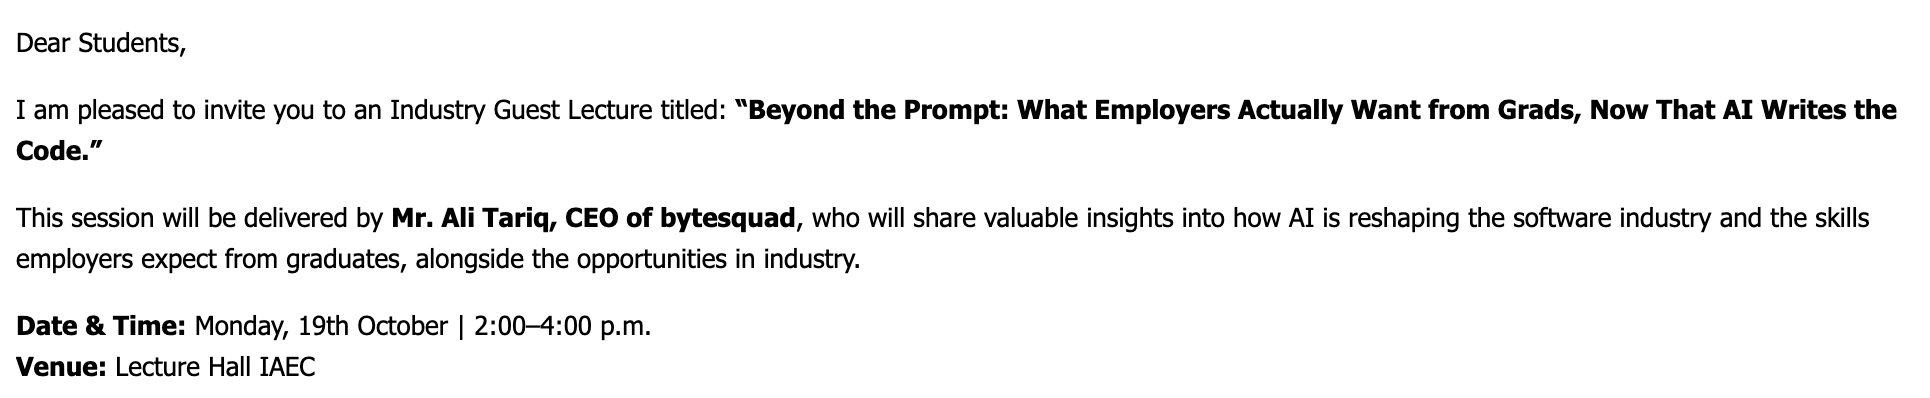
\includegraphics[width=1.0\textwidth]{images/criterion_3/media/guest-lecture.png} }
\caption{Recent Industry Talk Invite Example}
\label{fig:talk}
\end{figure}
%-----------------------------------------------------------------------

\hypertarget{sec:4.8internship}{%
\section{Internship Program}\label{sec:4.8internship}}

A comprehensive internship program has been developed to provide SEECS and SE students hands-on training in working on industrial problems. Every summer, the department, SEECS ILO, and NUST Placement Office (NPO) facilitate second and third year students to secure internships with leading software companies and government agencies. Figure~\ref{figure:Outline_of_internship_program_at_SEECS} shows the process. After the 4th semester, students contact the ILO for internship placement. After completing the requirements of mandatory 6-8 week internship, the students complete the employer survey and submit proof of attendance, verified by the ILO and the employer. The students then submit their internship report, followed by an internship interview conducted by the Internship Assessment Committee (IAC) members. The IAC Head compiles the results and present them to the DBS. Finally these are made available to students through NIRS. Table~\ref{tab:Hierarchy_of_Internship_Assessment_Committee} shows the IAC hierarchy and responsibilities.


\begin{figure}[H]
\centering
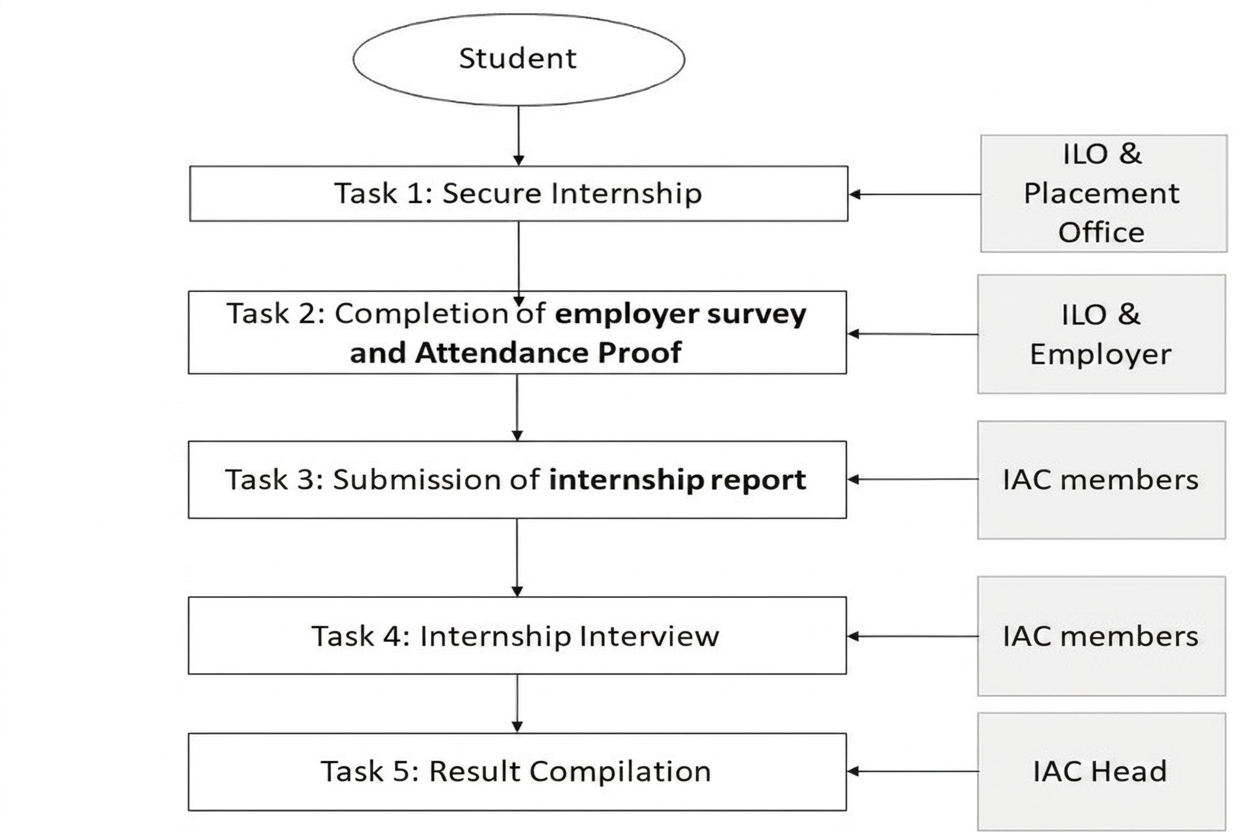
\includegraphics[width=1.0\textwidth]{images/criterion_3/media/img_internship_process.jpeg} % <-- Increased to 100%
\caption{Outline of internship program at SEECS}
\label{figure:Outline_of_internship_program_at_SEECS}
\end{figure}

\begin{table}[H]
\centering
\footnotesize % <-- Reduces font size
\renewcommand{\arraystretch}{0.85} % <-- Tightens vertical row spacing
\caption{Hierarchy of Internship Assessment Committee}
\label{tab:Hierarchy_of_Internship_Assessment_Committee}
\begin{tabular}{>{\raggedright\arraybackslash}p{0.30\textwidth}
                >{\raggedright\arraybackslash}p{0.52\textwidth}}
\toprule
\textbf{Position} & \textbf{Role} \\
\midrule
IAC Head & Overall oversight and custodian of evaluation records \\
ILO (Industry Liaison Officer) & First point of contact for students; IAC member \\
IAC Members & Evaluation and interview of internees \\
\bottomrule
\end{tabular}
\end{table}

The internship feedback forms were revised recently to obtain indirect assessment of PLOs from the employers of interns. The detailed analysis of PLO attainment based on internship feedback for the 2K21, 2K22, and 2K23 batches has already been presented in Section~\ref{sec:internshipfeedback}. The results presented in that section provide evidence of PLO attainment based on employer feedback. Table~\ref{tab:Summary_of_Students_from_Different_Batches_under_the_SEECS_Internship_Program} provides a summary of students who have successfully completed summer internships. BESE 2K23 is currently under evaluation but 24 have already successfully completed the entire process.

\begin{table}[H]
\centering
\footnotesize % <-- Reduces font size
\renewcommand{\arraystretch}{0.85} % <-- Tightens vertical row spacing
\caption{Batch-wise Summary of Students Completing Internship Program}
\label{tab:Summary_of_Students_from_Different_Batches_under_the_SEECS_Internship_Program}
\begin{tabular}{>{\raggedright\arraybackslash}p{0.30\textwidth}
                >{\centering\arraybackslash}p{0.25\textwidth}}
\toprule
\textbf{Batch} & \textbf{No.\ of Completed Internships} \\
\midrule
BESE 2K21 & 85 \\
BESE 2K22 & 81 \\
BESE 2K23 & 24 \\
\midrule
\textbf{Total} & \textbf{190} \\
\bottomrule
\end{tabular}
\end{table}

\hypertarget{sec:4.9othermethods}{%
\section{Additional Learning Methods}\label{sec:4.9othermethods}}

NUST SEECS provides students with various opportunities to participate in workshops, training programs, seminars, and short courses. Some of these activities are presented in Table~\ref{tab:Workshops_Training_Programs_Seminars_and_Short_Courses}. These activities enhance academic, technical, and research competencies while providing exposure to emerging technologies and industry trends. They also promote interaction with academic and industry experts contributing to continuous improvement of the academic programs.  Additionally, regular language courses are also offered to facilitate students aiming to pursue higher education or work abroad. These courses include \emph{Arabic, French, and German}. 

\begin{table}[H]
\centering
\footnotesize % <-- Reduces font size
\renewcommand{\arraystretch}{0.85} % <-- Tightens vertical row spacing
\caption{Workshops Training Programs Seminars and Short Courses}
\label{tab:Workshops_Training_Programs_Seminars_and_Short_Courses}
\begin{tabular}{c p{2cm} p{5.5cm} p{3cm}}
\toprule
\textbf{\begin{tabular}[c]{@{}c@{}}Sr.\\ No.\end{tabular}} & \textbf{Type} & \textbf{Title} & \textbf{Date} \\ 
\midrule

1 & Workshop & Building Capacity with AI for Sustainable Ventures & November 19, 2025 \\ \addlinespace

2 & Workshop & Reinforcement Learning Unleashed: Hands-On Skill Building for Smarter AI & August 18-22, 2025 \\ \addlinespace

3 & Workshop & Resilient Futures: GeoAI for Farms \& SLUMs---Robotics and Remote Sensing for Pakistan's Sustainable Well-Being & October 9, 2025 \\ \addlinespace

4 & Training Program & Programming for AI Systems & July 8, 2024 - September 8, 2024 \\ \addlinespace

5 & Seminar & Unlocking Business Value with AI and Data Analytics & May 2, 2024 \\ \addlinespace

6 & Workshop & FinTech Frontier: Harnessing the Power of LLMs & February 21-23, 2024 \\ \addlinespace

7 & Short Course & A four day short course on Sensors and AI & June 5-8, 2023 \\ 

\bottomrule
\end{tabular}
\end{table}

\begin{comment}
\hypertarget{sec:4.10assessment}{%
\section{Assessment of Learning Outcomes}\label{sec:4.10assessment}}

{\color{red}The learning outcomes at both course level and program level are measured in a direct and indirect manner, described in detail in Criterion~2 (Sections~3.6.1 to~3.6.4).}

\hypertarget{sec:gaattainment}{%
\subsection{Attainment of Graduate Attributes (GAs)}\label{sec:gaattainment}}

The BESE curriculum ensures coverage of all Knowledge, Skills, and Attitude (KSA) domains across the eleven graduate attributes (PLOs). Graduate attribute attainment is measured at graduation level through direct assessment (coursework and FYDP rubrics) and indirect assessment (exit surveys and internship feedback), as described in Criterion~2.
\end{comment}


%\begin{figure}[H]
%\centering
%\includegraphics[width=\textwidth]{images/criterion_3/media/image16.png}
%\missingcriterionthreefigure{image16.png}
%\end{figure}


%-----------------------------------------------------------------------
\hypertarget{sec:4.11fydp}{%
\section{Final Year Design Projects}\label{sec:4.11fydp}}

The BESE program includes a Final Year Design Project (FYDP) which is a design/research-oriented activity spanning the last two semesters and serving as the pinnacle activity for inculcating desired graduate attributes through solutions to complex engineering problems, guided by the FYDP policy (Annexure~\ref{app:criteria-3_FYP_Guidelines}). The FYDP is evaluated through oral presentation, documentation, and poster design across proposal defense, mid-defense, open house, and final defense with the complete evaluation process outlined in Annexure~\ref{app:criteria-3_FYP_Guidelines} and OBE-based assessment described in Section~\ref{sec:FYDP}

\begin{comment}
\begin{figure}[H]
\centering
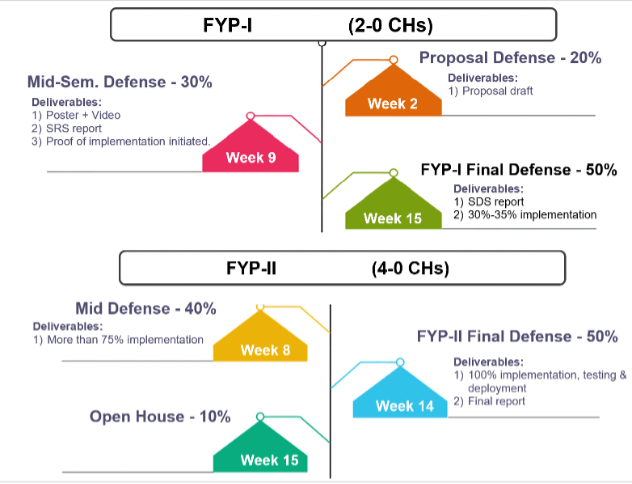
\includegraphics[width=0.8\textwidth]{images/criterion_3/media/img_fydp_process.png}
\caption{Roadmap of Final Year Design Project}
\label{figure:Roadmap_of_Final_Year_Design_Project}
\end{figure}
\end{comment}

The FYDP assessments shown in Figure~\ref{figure:fydp1} provide direct evaluation of PLOs. The PLO mapping for each FYDP semester (7 \& 8) of Batch 2k23 is listed in Table~\ref{tab:Mapping_of_FYDP_to_Direct_Assessment_of_PLOs-12} while the PLO mapping for the subsequent batches is shown in Table~\ref{tab:Mapping_of_FYDP_to_Direct_Assessment_of_PLOs-11}. Each activity is measured through rubrics which are shared with students at project initiation (Annexure~\ref{app:criteria-3_FYP_Guidelines}). Mid-defense, final report, and final presentation evaluations are conducted by a committee comprising of domain experts (relevant faculty members). The marks obtained in each activity stage are recorded in TMS and are used for final result compilation. Table~\ref{tab:distribution} shows percentage weightage of each activity in FYDP assessment. Best Industrial Project and Overall Best Project for Rector's Gold Medal are selected at the end of FYDP via a competitive process where shortlisted projects undergo a final round of presentation and evaluation by two separate committees. 

\begin{figure}[H]
\centering
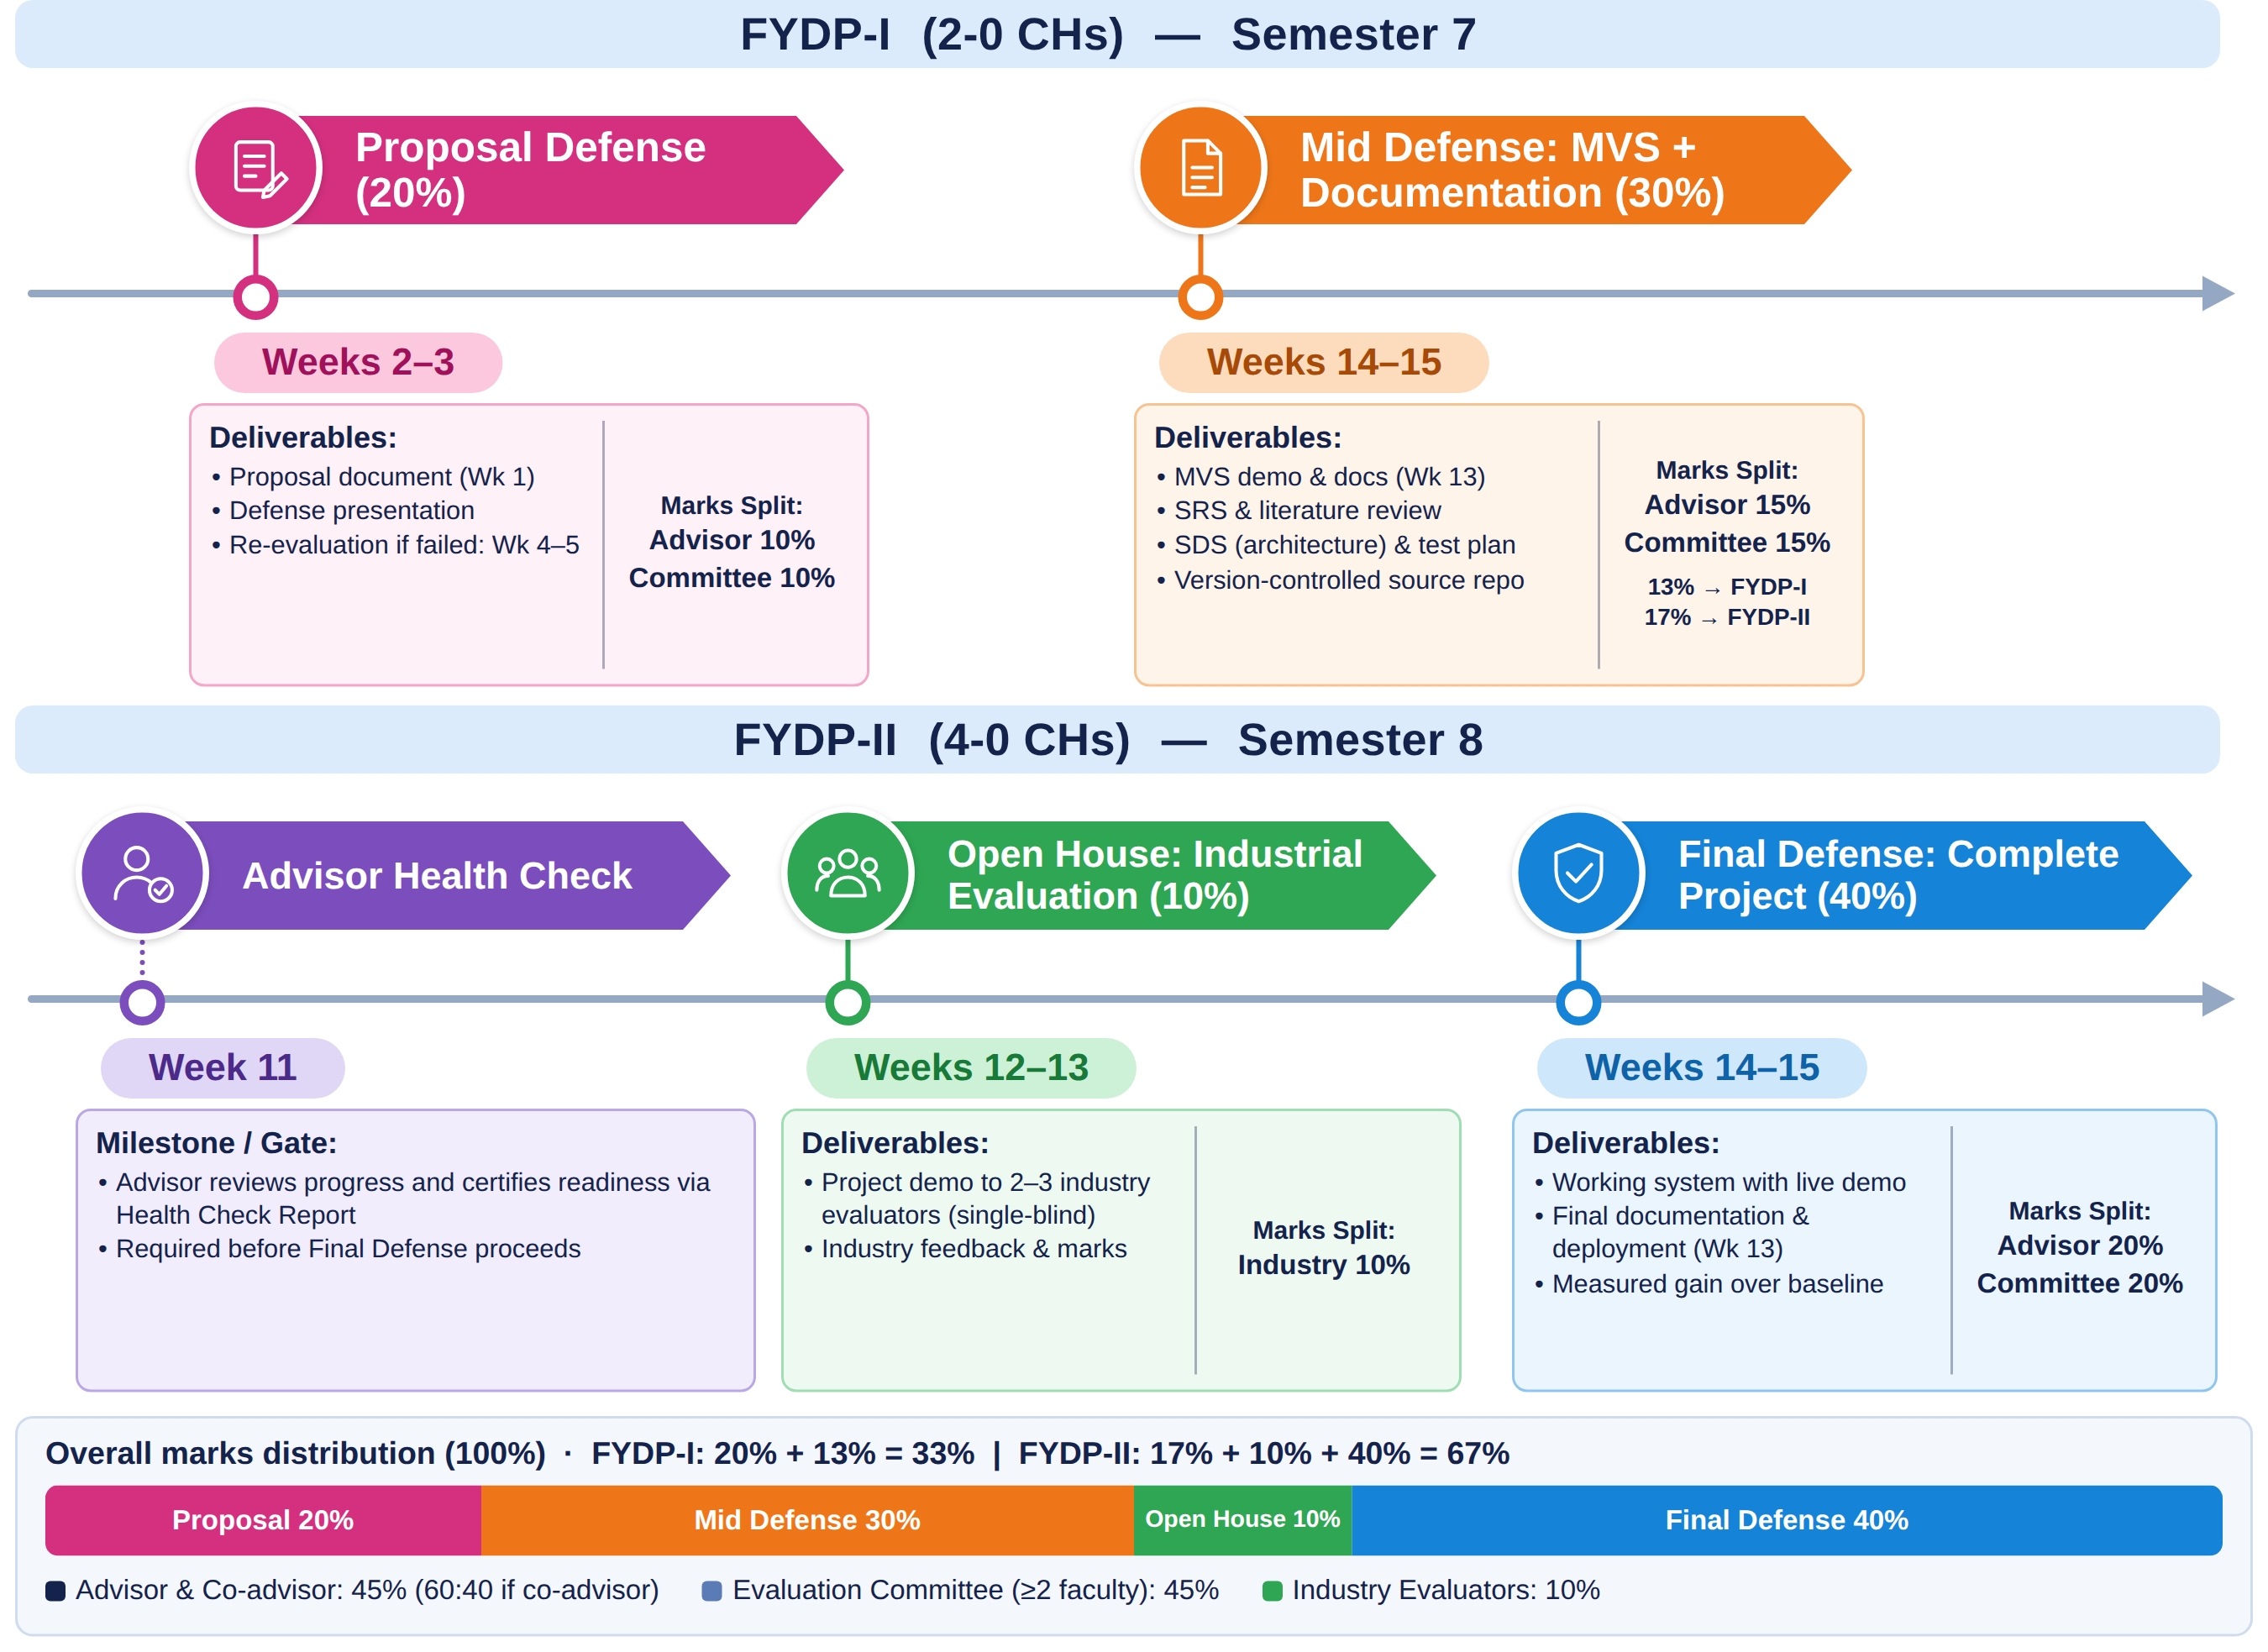
\includegraphics[width=0.9\textwidth]{images/criterion_2/media/FYDP-timeline.png}
\caption{Roadmap of Final Year Design Project (FYDP) Across 7\textsuperscript{th} \& 8\textsuperscript{th} Semesters.}
\label{figure:fydp1}
\end{figure}


\begin{comment}
\begin{landscape}
\begingroup\scriptsize\setlength{\tabcolsep}{3pt}
\begin{longtable}{>{\raggedright\arraybackslash}p{0.07\linewidth}
                  >{\raggedright\arraybackslash}p{0.18\linewidth}
                  >{\centering\arraybackslash}p{0.058\linewidth}
                  >{\centering\arraybackslash}p{0.058\linewidth}
                  >{\centering\arraybackslash}p{0.058\linewidth}
                  >{\centering\arraybackslash}p{0.058\linewidth}
                  >{\centering\arraybackslash}p{0.058\linewidth}
                  >{\centering\arraybackslash}p{0.058\linewidth}
                  >{\centering\arraybackslash}p{0.058\linewidth}
                  >{\centering\arraybackslash}p{0.058\linewidth}
                  >{\centering\arraybackslash}p{0.058\linewidth}
                  >{\centering\arraybackslash}p{0.058\linewidth}
                  >{\centering\arraybackslash}p{0.058\linewidth}}
\caption{Mapping of FYDP to Direct Assessment of PLOs} \\
\label{tab:Mapping_of_FYDP_to_Direct_Assessment_of_PLOs} \\
\toprule
\textbf{Course} & \textbf{Title} & \textbf{PLO 1} & \textbf{PLO 2} & \textbf{PLO 3} & \textbf{PLO 4} & \textbf{PLO 5} & \textbf{PLO 6} & \textbf{PLO 7} & \textbf{PLO 8} & \textbf{PLO 9} & \textbf{PLO 10} & \textbf{PLO 11} \\
& & \scriptsize Eng.Know. & \scriptsize Prob.Anal. & \scriptsize Design/Dev. & \scriptsize Invest. & \scriptsize Tool Usage & \scriptsize Eng.\&World & \scriptsize Ethics & \scriptsize Teamwork & \scriptsize Commun. & \scriptsize Proj.Mgmt. & \scriptsize Lifelong \\
\midrule
\endfirsthead
\multicolumn{13}{l}{\footnotesize\textit{Continued from previous page}} \\
\toprule
\textbf{Course} & \textbf{Title} & \textbf{1} & \textbf{2} & \textbf{3} & \textbf{4} & \textbf{5} & \textbf{6} & \textbf{7} & \textbf{8} & \textbf{9} & \textbf{10} & \textbf{11} \\
\midrule
\endhead
\bottomrule
\endlastfoot
SE-498 & Final Year Design Project -- I  & $\checkmark$ & $\checkmark$ & $\checkmark$ & $\checkmark$ & $\checkmark$ & $\checkmark$ & $\checkmark$ & $\checkmark$ & $\checkmark$ & $\checkmark$ & \\
SE-499 & Final Year Design Project -- II & $\checkmark$ & $\checkmark$ & $\checkmark$ & $\checkmark$ & $\checkmark$ & $\checkmark$ & $\checkmark$ & $\checkmark$ & $\checkmark$ & $\checkmark$ & $\checkmark$ \\
\end{longtable}
\endgroup
\end{landscape}
\end{comment}

\begin{table}[H]
\centering
\footnotesize % <-- Keeps size compact
\renewcommand{\arraystretch}{0.85} % <-- Tightens vertical padding
\caption{Mapping of FYDP to Direct Assessment of PLOs for 2K23 Batch (12-PLOs)}
\label{tab:Mapping_of_FYDP_to_Direct_Assessment_of_PLOs-12}
\begin{tabular}{c >{\raggedright\arraybackslash}p{0.42\textwidth} >{\centering\arraybackslash}p{0.18\textwidth} >{\centering\arraybackslash}p{0.18\textwidth}}
\toprule
\textbf{PLO \#} & \textbf{Program Learning Outcome} & \textbf{SE-498 (FYDP -- I)} & \textbf{SE-499 (FYDP -- II)} \\
\midrule
PLO 1  & Engineering Knowledge              & $\checkmark$ & $\checkmark$ \\
PLO 2  & Problem Analysis                   & $\checkmark$ & $\checkmark$ \\
PLO 3  & Design/Development of Solutions    & $\checkmark$ & $\checkmark$ \\
PLO 4  & Investigation                      & $\checkmark$ & $\checkmark$ \\
PLO 5  & Modern Tool Usage                  & $\checkmark$ & $\checkmark$ \\
PLO 6  & Engineer and Society      & $\checkmark$ & $\checkmark$ \\
PLO 7  & Environment and Sustainability        & $\checkmark$ & $\checkmark$ \\
PLO 8  & Ethics                             &  & $\checkmark$ \\
PLO 9  & Individual and Teamwork            & $\checkmark$ & $\checkmark$ \\
PLO 10  & Communication                      & $\checkmark$ & $\checkmark$ \\
PLO 11 & Project Management                 & $\checkmark$ & $\checkmark$ \\
PLO 12 & Lifelong Learning                  &              & $\checkmark$ \\
\bottomrule
\end{tabular}
\end{table}

\begin{table}[H]
\centering
\footnotesize % <-- Keeps size compact
\renewcommand{\arraystretch}{0.85} % <-- Tightens vertical padding
\caption{Mapping of FYDP to Direct Assessment of PLOs for 2K24 \& Onwards Batches (11-PLOs)}
\label{tab:Mapping_of_FYDP_to_Direct_Assessment_of_PLOs-11}
\begin{tabular}{c >{\raggedright\arraybackslash}p{0.42\textwidth} >{\centering\arraybackslash}p{0.18\textwidth} >{\centering\arraybackslash}p{0.18\textwidth}}
\toprule
\textbf{PLO \#} & \textbf{Program Learning Outcome} & \textbf{SE-498 (FYDP -- I)} & \textbf{SE-499 (FYDP -- II)} \\
\midrule
PLO 1  & Engineering Knowledge              & $\checkmark$ & $\checkmark$ \\
PLO 2  & Problem Analysis                   & $\checkmark$ & $\checkmark$ \\
PLO 3  & Design/Development of Solutions    & $\checkmark$ & $\checkmark$ \\
PLO 4  & Investigation                      & $\checkmark$ & $\checkmark$ \\
PLO 5  & Modern Tool Usage                  & $\checkmark$ & $\checkmark$ \\
PLO 6  & Engineer and Society       & $\checkmark$ & $\checkmark$ \\
PLO 7  & Ethics                             &  & $\checkmark$ \\
PLO 8  & Individual and Teamwork            & $\checkmark$ & $\checkmark$ \\
PLO 9  & Communication                      & $\checkmark$ & $\checkmark$ \\
PLO 10 & Project Management                 & $\checkmark$ & $\checkmark$ \\
PLO 11 & Lifelong Learning                  &              & $\checkmark$ \\
\bottomrule
\end{tabular}
\end{table}

\begin{table}[H]
\centering
\footnotesize % <-- Reduces font size
\renewcommand{\arraystretch}{0.85} % <-- Tightens vertical row spacing
\caption{Percentage of Weightage for Each FYDP Activity}
\label{tab:distribution}
\begin{tabular}{>{\raggedright\arraybackslash}p{0.30\textwidth}
                >{\centering\arraybackslash}p{0.25\textwidth}}
\toprule
\textbf{Activity} & \textbf{Percentage} \\
\midrule
Proposal Defense & 20\% \\
Mid Defense-I & 13\% \\
Mid Defense-II & 17\% \\
Open House & 10\% \\
Final Defense & 40\%\\
\midrule
\textbf{Total} & \textbf{100\%} \\
\bottomrule
\end{tabular}
\end{table}


\hypertarget{sec:fydpsdg}{%
\subsection{Mapping of FYDPs with UN SDGs}\label{sec:fydpsdg}}

All final year projects in the BESE program are mandatorily mapped to at least one UN Sustainable Development Goal (SDG), reflecting the program's commitment to socially responsible innovation and instilling in graduates a sense of global responsibility to address pressing challenges through software engineering. This ensures that projects demonstrate both technical proficiency and contribution to sustainability, equity, and social progress. The mapping of BESE-2K22 FYDPs to relevant UN SDGs is shown in Table~\ref{tab:Mapping_of_FYDPs_to_SDGs_for_BESE_Batch}. List of sample projects is presented in Annexure~\ref{app:criteria-3_List of FYDP BESE 2K22 Batch}.

\begin{comment}
\begin{table}[H]
\centering
\footnotesize % <-- Reduces font size
\renewcommand{\arraystretch}{0.85} % <-- Tightens vertical row spacing
\caption{Mapping of FYDPs to SDGs for BESE ?? Batch (BESE-??)}
\label{tab:Mapping_of_FYDPs_to_SDGs_for_BESE_Batch}
\begin{tabular}{>{\centering\arraybackslash}p{0.08\textwidth}
                >{\raggedright\arraybackslash}p{0.48\textwidth}
                >{\centering\arraybackslash}p{0.24\textwidth}}
\toprule
\textbf{S.No.} & \textbf{SDG} & \textbf{Number of Projects} \\
\midrule
1  & No Poverty & 0 \\
2  & Zero Hunger & 0 \\
3  & Good Health and Well-Being & 14 \\
4  & Quality Education & 7 \\
5  & Gender Equality & 2 \\
6  & Clean Water and Sanitation & 0 \\
7  & Affordable and Clean Energy & 0 \\
8  & Decent Work and Economic Growth & 7 \\
9  & Industry, Innovation and Infrastructure & 15 \\
10 & Reduced Inequalities & 2 \\
11 & Sustainable Cities and Communities & 7 \\
12 & Responsible Consumption and Production & 4 \\
13 & Climate Action & 5 \\
14 & Life Below Water & 0 \\
15 & Life on Land & 1 \\
16 & Peace, Justice and Strong Institutions & 3 \\
17 & Partnerships for Goals & 0 \\
\midrule
   & \textbf{Total Number of Projects} & \textbf{37} \\
\bottomrule
\end{tabular}
\end{table}
\end{comment}

\begin{table}[H]
\centering
\footnotesize
\renewcommand{\arraystretch}{0.85}
\caption{No. of FYDPs (BESE 2K22) Mapped to Relevant SDGs}
\label{tab:Mapping_of_FYDPs_to_SDGs_for_BESE_Batch}

\begin{tabular}{>{\centering\arraybackslash}p{0.08\textwidth}
                >{\raggedright\arraybackslash}p{0.48\textwidth}
                >{\centering\arraybackslash}p{0.24\textwidth}}
\toprule
\textbf{S.No.} & \textbf{SDG} & \textbf{Number of Projects} \\
\midrule

1  & No Poverty & 4 \\
2  & Zero Hunger & 3 \\
3  & Good Health and Well-Being & 11 \\
4  & Quality Education & 15 \\
5  & Gender Equality & 1 \\
6  & Clean Water and Sanitation & 1 \\
7  & Affordable and Clean Energy & 0 \\
8  & Decent Work and Economic Growth & 9 \\
9  & Industry, Innovation and Infrastructure & 17 \\
10 & Reduced Inequalities & 1 \\
11 & Sustainable Cities and Communities & 4 \\
12 & Responsible Consumption and Production & 6 \\
13 & Climate Action & 1 \\
14 & Life Below Water & 0 \\
15 & Life on Land & 0 \\
16 & Peace, Justice and Strong Institutions & 2 \\
17 & Partnerships for Goals & 0 \\

\bottomrule
\end{tabular}
\end{table}

\begin{comment}
{\footnotesize
\renewcommand{\arraystretch}{0.85}
\begin{longtable}{>{\centering\arraybackslash}p{0.08\textwidth}
                  >{\raggedright\arraybackslash}p{0.68\textwidth}
                  >{\centering\arraybackslash}p{0.10\textwidth}}
\caption{FYDP Projects -- BESE 2K22 Batch} \\
\toprule
\textbf{Sr.\#} & \textbf{Project Title} & \textbf{Dept.} \\
\midrule
\endfirsthead
\multicolumn{3}{l}{\footnotesize\textit{Continued from previous page}} \\
\toprule
\textbf{Sr.\#} & \textbf{Project Title} & \textbf{Dept.} \\
\midrule
\endhead
\midrule \multicolumn{3}{r}{\footnotesize\textit{Continued on next page}} \\
\endfoot
\bottomrule
\endlastfoot
1  & AI Based Security Orchestration, Automation, and Response System & SE \\
2  & OBE Assess: AI-Powered Outcome-Based Education Assessment System & SE \\
3  & CyberShield: Cybersecurity Awareness \& Incident Reporting Portal & SE \\
4  & Non-Technical Cofounder Super Agent (E-commerce) & SE \\
5  & HRXpert: Automating Talent Acquisition with Artificial Intelligence & SE \\
6  & EEGWriter: Multimodal Deep Learning Framework for Automated EEG Diagnostic Report Generation & SE \\
7  & AI-Driven UAV System for Disaster Response and Real-Time Rescue Operations & SE \\
8  & From Drones to Decisions: LLM-Based Crop Health Insights from RGB and Multispectral Data & SE \\
9  & Explainable AI for EEG Signal Classification (NeuroXplain) & SE \\
10 & EmergeOS: Autonomy-as-a-Service & SE \\
11 & Smart AgriAssist: AI-Powered Crop Disease Detection and Market Advisory System for Small Farmers in Pakistan & SE \\
12 & Disrupting Deepfake Generation Through Adversarial Attacks & SE \\
13 & Troubleshooting Copilot & SE \\
14 & Artificial Intelligence-Based End Point Detection and Response System & SE \\
15 & AI-Powered Profitability Estimation for Short-Term Rental Properties & SE \\
16 & Sedata.AI & SE \\
17 & Gaze-Guided Explainable AI for EEG-Based Brain Disorder Classification & SE \\
18 & SmartSketch: AI-Powered Facial Image Generator from Natural Language Descriptions & SE \\
19 & A Hybrid AI Framework for Dynamic Behavioral Adaptation & SE \\
20 & An Expert-Guided Multimodal AI Ecosystem for Diagnostic Intelligence & SE \\
21 & Smart Parental Control \& Monitoring System for Child Devices & SE \\
22 & Callisto AI: Conversational Intelligent CI/CD Automation Tool & SE \\
23 & AI-Assisted Forensic Analysis System for Decision Support & SE \\
24 & Cloud Optimization: Cost and Security for Enterprise Success & SE \\
25 & LiDAR-Based Plant Phenotyping for Precision Agriculture & SE \\
26 & Adaptive Web Interaction: Leveraging Reinforcement Learning for Comprehensive Action Support & SE \\
27 & FleaderAI: An AI-Driven End-to-End Lead Relationship Automation via Memory-Centric Conversational Agents & SE \\
28 & Emotion Detection from Micro-Expressions & SE \\
29 & Design and Development of a Decentralized B2B2C Platform for Skilled Labour Connectivity & SE \\
30 & InnBotics & SE \\
31 & HunarmandAI: Culturally-Aware Intelligent Tutoring for Low-Literacy Urdu Speakers & SE \\
32 & AI-Tutor for University Entry Test Preparation & SE \\
33 & Federated Data Lakes and Intelligent Healthcare Management for Pakistan & SE \\
34 & TaxSimplify: Automated Budgeting \& Tax Return Filing System & SE \\
\end{longtable}
}
\end{comment}

\subsection{Mapping of FYDPs with CEP Attributes}
\label{sec:fydpcep}
The Final Year Design Projects (FYDPs) are structured to provide students with opportunities to apply engineering knowledge and professional skills to complex, real-world software engineering problems. Table~\ref{tab:fydp_cep_mapping} presents the mapping of FYDP requirements and activities with the relevant CEP attributes.

\begin{table}[H]
\centering
\scriptsize % <-- Reduced font size from \footnotesize to \scriptsize
\renewcommand{\arraystretch}{0.70} % <-- Tightened vertical padding further
\caption{Mapping of FYDPs with CEP Attributes}
\label{tab:fydp_cep_mapping}
\begin{tabular}{>{\raggedright\arraybackslash}p{0.18\textwidth}
                >{\raggedright\arraybackslash}p{0.20\textwidth}
                >{\raggedright\arraybackslash}p{0.22\textwidth}
                >{\raggedright\arraybackslash}p{0.24\textwidth}}
\toprule
\textbf{Engineering Design Requirement} & 
\textbf{Evidence in FYDP Guidelines (Annex X)} & 
\textbf{Relevant Washington Accord WP(s)} & 
\textbf{Remarks} \\
\midrule

Problem Identification & 
Problem Definition chapter in Final Report Template & 
WP1 -- Depth of knowledge required, WP2 -- Conflicting requirements & 
Students identify, analyze, and justify a real-world engineering problem with multiple stakeholder needs and constraints. \\ \addlinespace[2pt]

Requirements Engineering & 
Software Requirements Specification (SRS) Template & 
WP2 -- Conflicting requirements, WP3 -- Depth of analysis required & 
Functional and non-functional requirements are elicited, analyzed, prioritized, and documented before implementation. \\ \addlinespace[2pt]

System Design & 
System Architecture and Detailed Design chapters & 
WP4 -- Familiarity of issues, WP5 -- Extent of applicable codes, WP6 -- Stakeholder involvement & 
Students design system architectures and components while considering standards, constraints, and stakeholder expectations. \\ \addlinespace[2pt]

Engineering Analysis & 
Methodology and Literature Review chapters & 
WP1 -- Depth of knowledge required, WP3 -- Depth of analysis required & 
Selection of algorithms, methodologies, tools, and technologies is justified through critical analysis and literature review. \\ \addlinespace[2pt]

System Implementation & 
Implementation \& Testing chapter & 
WP3 -- Depth of analysis required, WP7 -- Interdependence & 
The complete engineering solution is developed by integrating multiple software components and technologies. \\ \addlinespace[2pt]

System Validation & 
Results \& Discussion chapter & 
WP2 -- Conflicting requirements, WP7 -- Interdependence & 
The solution is verified and validated against the original requirements using appropriate testing and evaluation techniques. \\ \addlinespace[2pt]

Engineering Documentation & 
Standard report templates & 
WP5 -- Extent of applicable codes, WP6 -- Stakeholder involvement & 
The entire engineering design process is documented according to departmental templates, standards, and professional practices. \\

\bottomrule
\end{tabular}
\end{table}

%-----------------------------------------------------------------------
\hypertarget{sec:4.13grades}{%
\section{Grade Distribution}\label{sec:4.13grades}}

The Software Engineering Department at NUST-SEECS follow a relative grading system that uses A, B+, B, C+, C, D+, D, and F grades. The grade-wise distribution of results for all active BESE batches for the Spring~2026 End-Semester Examination is presented in Annexure~\ref{app:criteria-3_System of instruction and examination}. Details of the system are discussed in Section~\ref{sec:performance-evaluation}.
\begin{comment}
\clearpage
\begin{landscape}
\begingroup\scriptsize\setlength{\tabcolsep}{3pt}
\begin{longtable}{>{\raggedright\arraybackslash}p{0.08\linewidth}
                  >{\raggedright\arraybackslash}p{0.28\linewidth}
                  >{\centering\arraybackslash}p{0.047\linewidth}
                  >{\centering\arraybackslash}p{0.047\linewidth}
                  >{\centering\arraybackslash}p{0.047\linewidth}
                  >{\centering\arraybackslash}p{0.047\linewidth}
                  >{\centering\arraybackslash}p{0.047\linewidth}
                  >{\centering\arraybackslash}p{0.047\linewidth}
                  >{\centering\arraybackslash}p{0.047\linewidth}
                  >{\centering\arraybackslash}p{0.047\linewidth}
                  >{\centering\arraybackslash}p{0.047\linewidth}
                  >{\centering\arraybackslash}p{0.06\linewidth}}
\caption{Grade Distribution -- Intake Batch UG SE-2K22, ESE Spring 2026} \\
\toprule
\textbf{Course Code} & \textbf{Course Name} & \textbf{Total} & \textbf{A} & \textbf{B+} & \textbf{B} & \textbf{C+} & \textbf{C} & \textbf{D+} & \textbf{D} & \textbf{F} & \textbf{Remarks} \\
\midrule
\endfirsthead
\multicolumn{12}{l}{\footnotesize\textit{Continued from previous page}} \\
\toprule
\textbf{Course Code} & \textbf{Course Name} & \textbf{Total} & \textbf{A} & \textbf{B+} & \textbf{B} & \textbf{C+} & \textbf{C} & \textbf{D+} & \textbf{D} & \textbf{F} & \textbf{Rem.} \\
\midrule
\endhead
\bottomrule
\endlastfoot
CSL-402 & Community Service Learning A & 43 & 0 & 0 & 0 & 0 & 0 & 0 & 0 & 0 & Q \\
CSL-402 & Community Service Learning B & 43 & 0 & 0 & 0 & 0 & 0 & 0 & 0 & 0 & Q \\
CS-481  & Computer Forensics (A)       & 54 & 5 & 14 & 16 & 11 & 4 & 4 & 0 & 0 & \\
CS-416  & Large Language Models (Gp-01) & 47 & 8 & 10 & 13 & 7 & 5 & 2 & 2 & 0 & \\
CS-416  & Large Language Models (Gp-02) & 20 & 2 & 2 & 2 & 6 & 5 & 2 & 1 & 0 & \\
CS-415  & Mobile Application Development & 52 & 6 & 10 & 17 & 10 & 6 & 3 & 0 & 0 & \\
SE-499  & Final Year Design Project -- II & 85 & 69 & 16 & 0 & 0 & 0 & 0 & 0 & 0 & \\
\end{longtable}

\begin{longtable}{>{\raggedright\arraybackslash}p{0.08\linewidth}
                  >{\raggedright\arraybackslash}p{0.28\linewidth}
                  >{\centering\arraybackslash}p{0.045\linewidth}
                  >{\centering\arraybackslash}p{0.045\linewidth}
                  >{\centering\arraybackslash}p{0.045\linewidth}
                  >{\centering\arraybackslash}p{0.045\linewidth}
                  >{\centering\arraybackslash}p{0.045\linewidth}
                  >{\centering\arraybackslash}p{0.045\linewidth}
                  >{\centering\arraybackslash}p{0.045\linewidth}
                  >{\centering\arraybackslash}p{0.045\linewidth}
                  >{\centering\arraybackslash}p{0.045\linewidth}
                  >{\centering\arraybackslash}p{0.045\linewidth}}
\caption{Grade Distribution -- Intake Batch UG SE-2K23, ESE Spring 2026} \\
\toprule
\textbf{Code} & \textbf{Course Name} & \textbf{Total} & \textbf{A} & \textbf{B+} & \textbf{B} & \textbf{C+} & \textbf{C} & \textbf{D+} & \textbf{D} & \textbf{F} & \textbf{XF} \\
\midrule
\endfirsthead
\multicolumn{12}{l}{\footnotesize\textit{Continued}} \\
\toprule
\textbf{Code} & \textbf{Course Name} & \textbf{Total} & \textbf{A} & \textbf{B+} & \textbf{B} & \textbf{C+} & \textbf{C} & \textbf{D+} & \textbf{D} & \textbf{F} & \textbf{XF} \\
\midrule
\endhead
\bottomrule
\endlastfoot
MGT-271 & Entrepreneurship A & 44 & 6 & 15 & 21 & 2 & 0 & 0 & 0 & 0 & \\
MGT-271 & Entrepreneurship B & 41 & 5 & 21 & 15 & 0 & 0 & 0 & 0 & 0 & \\
SE-320  & Formal Methods A   & 44 & 7 & 9  & 12 & 10 & 4 & 1 & 0 & 1 & \\
SE-320  & Formal Methods B   & 41 & 6 & 12 & 16 & 6  & 1 & 0 & 0 & 0 & \\
CS-261  & Human Computer Interaction A & 44 & 2 & 13 & 16 & 9 & 3 & 0 & 1 & 0 & \\
CS-261  & Human Computer Interaction B & 41 & 4 & 16 & 15 & 6 & 0 & 0 & 0 & 0 & \\
CS-471  & Machine Learning A & 47 & 5 & 8  & 11 & 11 & 6 & 2 & 2 & 2 & \\
CS-471  & Machine Learning B & 43 & 3 & 13 & 17 & 5  & 2 & 1 & 1 & 1 & \\
SE-430  & Software Project Management A & 44 & 5 & 13 & 12 & 10 & 2 & 2 & 0 & 0 & \\
SE-430  & Software Project Management B & 43 & 4 & 14 & 17 & 6  & 2 & 0 & 0 & 0 & \\
SE-321  & Software Quality Engineering A & 44 & 4 & 8  & 10 & 12 & 7 & 2 & 0 & 1 & \\
SE-321  & Software Quality Engineering B & 42 & 5 & 11 & 16 & 7  & 3 & 0 & 0 & 0 & \\
\end{longtable}

\begin{longtable}{>{\raggedright\arraybackslash}p{0.08\linewidth}
                  >{\raggedright\arraybackslash}p{0.28\linewidth}
                  >{\centering\arraybackslash}p{0.043\linewidth}
                  >{\centering\arraybackslash}p{0.043\linewidth}
                  >{\centering\arraybackslash}p{0.043\linewidth}
                  >{\centering\arraybackslash}p{0.043\linewidth}
                  >{\centering\arraybackslash}p{0.043\linewidth}
                  >{\centering\arraybackslash}p{0.043\linewidth}
                  >{\centering\arraybackslash}p{0.043\linewidth}
                  >{\centering\arraybackslash}p{0.043\linewidth}
                  >{\centering\arraybackslash}p{0.043\linewidth}
                  >{\centering\arraybackslash}p{0.043\linewidth}}
\caption{Grade Distribution -- Intake Batch UG SE-2K24, ESE Spring 2026} \\
\toprule
\textbf{Code} & \textbf{Course Name} & \textbf{Total} & \textbf{A} & \textbf{B+} & \textbf{B} & \textbf{C+} & \textbf{C} & \textbf{D+} & \textbf{D} & \textbf{F} & \textbf{XF} \\
\midrule
\endfirsthead
\multicolumn{12}{l}{\footnotesize\textit{Continued}} \\
\toprule
\textbf{Code} & \textbf{Course Name} & \textbf{Total} & \textbf{A} & \textbf{B+} & \textbf{B} & \textbf{C+} & \textbf{C} & \textbf{D+} & \textbf{D} & \textbf{F} & \textbf{XF} \\
\midrule
\endhead
\bottomrule
\endlastfoot
MATH-232 & Complex Variables and Transforms A & 45 & 7 & 10 & 12 & 4 & 3 & 3 & 3 & 2 & 1 \\
MATH-232 & Complex Variables and Transforms B & 42 & 6 & 7  & 11 & 4 & 5 & 3 & 2 & 2 & 2 \\
CS-251   & Design \& Analysis of Algorithms A & 45 & 5 & 10 & 13 & 5 & 9 & 2 & 1 & 0 & 0 \\
CS-251   & Design \& Analysis of Algorithms B & 40 & 4 & 6  & 10 & 8 & 6 & 4 & 0 & 0 & 1 \\
HU-101   & Islamic Studies A & 41 & 8 & 20 & 10 & 2 & 1 & 0 & 0 & 0 & 0 \\
HU-101   & Islamic Studies B & 40 & 4 & 18 & 14 & 4 & 0 & 0 & 0 & 0 & 0 \\
CS-330   & Operating Systems A & 46 & 7 & 15 & 11 & 9 & 1 & 2 & 0 & 0 & 1 \\
CS-330   & Operating Systems B & 40 & 6 & 13 & 9  & 7 & 3 & 1 & 1 & 0 & 0 \\
MATH-361 & Probability and Statistics A & 44 & 5 & 15 & 16 & 5 & 2 & 0 & 0 & 1 & 0 \\
MATH-361 & Probability and Statistics B & 41 & 6 & 8  & 12 & 7 & 3 & 2 & 0 & 2 & 1 \\
SE-211   & Software Design and Architecture A & 44 & 7 & 18 & 15 & 3 & 1 & 0 & 0 & 0 & 0 \\
SE-211   & Software Design and Architecture B & 38 & 3 & 10 & 19 & 4 & 1 & 1 & 0 & 0 & 0 \\
\end{longtable}

\begin{longtable}{>{\raggedright\arraybackslash}p{0.08\linewidth}
                  >{\raggedright\arraybackslash}p{0.30\linewidth}
                  >{\centering\arraybackslash}p{0.045\linewidth}
                  >{\centering\arraybackslash}p{0.045\linewidth}
                  >{\centering\arraybackslash}p{0.045\linewidth}
                  >{\centering\arraybackslash}p{0.045\linewidth}
                  >{\centering\arraybackslash}p{0.045\linewidth}
                  >{\centering\arraybackslash}p{0.045\linewidth}
                  >{\centering\arraybackslash}p{0.045\linewidth}
                  >{\centering\arraybackslash}p{0.045\linewidth}
                  >{\centering\arraybackslash}p{0.045\linewidth}}
\caption{Grade Distribution -- Intake Batch UG SE-2K25, ESE Spring 2026} \\
\toprule
\textbf{Code} & \textbf{Course Name} & \textbf{Total} & \textbf{A} & \textbf{B+} & \textbf{B} & \textbf{C+} & \textbf{C} & \textbf{D+} & \textbf{D} & \textbf{F} \\
\midrule
\endfirsthead
\multicolumn{11}{l}{\footnotesize\textit{Continued}} \\
\toprule
\textbf{Code} & \textbf{Course Name} & \textbf{Total} & \textbf{A} & \textbf{B+} & \textbf{B} & \textbf{C+} & \textbf{C} & \textbf{D+} & \textbf{D} & \textbf{F} \\
\midrule
\endhead
\bottomrule
\endlastfoot
EE-122   & Computer Architecture \& Logic Design A & 43 & 8 & 16 & 10 & 6 & 3 & 0 & 0 & 0 \\
EE-122   & Computer Architecture \& Logic Design B & 45 & 6 & 7  & 11 & 9 & 9 & 3 & 0 & 0 \\
MATH-161 & Discrete Mathematics A & 42 & 7 & 12 & 10 & 3 & 7 & 1 & 1 & 1 \\
MATH-161 & Discrete Mathematics B & 44 & 5 & 7  & 11 & 8 & 11 & 0 & 2 & 0 \\
HU-114   & Functional English A & 43 & 5 & 14 & 16 & 7 & 1 & 0 & 0 & 0 \\
HU-114   & Functional English B & 44 & 7 & 14 & 20 & 2 & 1 & 0 & 0 & 0 \\
MATH-121 & Linear Algebra and ODEs A & 45 & 9 & 7  & 14 & 3 & 2 & 5 & 2 & 2 \\
MATH-121 & Linear Algebra and ODEs B & 45 & 2 & 11 & 12 & 6 & 6 & 2 & 5 & 3 \\
CS-212   & Object Oriented Programming A & 44 & 7 & 7  & 16 & 9 & 2 & 1 & 2 & 0 \\
CS-212   & Object Oriented Programming B & 45 & 6 & 7  & 11 & 9 & 9 & 3 & 0 & 0 \\
HU-132   & Understanding of Quran-II A & 42 & 15 & 19 & 7 & 0 & 1 & 0 & 0 & 0 \\
HU-132   & Understanding of Quran-II B & 41 & 9  & 13 & 11 & 8 & 0 & 0 & 0 & 0 \\
\end{longtable}
\endgroup
\end{landscape}
\end{comment}
%=======================================================================





